\documentclass[class=4AM]{gymmureport}
% Für die Finale version, einfach das "draft" oben entfernen.

\addbibresource{My Library.bib}


\title{Messenger Software}
\subtitle{Verschlüsselte Kommunikation im lokalen Netzwerk oder Server}
\author{Luka Adjancic}
\klasse{4AM}
\advisor{Herr Geissmann}
\date{12. Oktober 2026}
\titleimage{picture-lib/titel-image.png}
\date{12.10.2026}



\begin{document}
\maketitle

\begin{abstract}
Die Kommunikation in einem lokalen Netzwerk ermöglicht einen schnellen Informationsaustausch, bringt jedoch hohe Risiken mit sich. Deshalb befasse ich mich in meiner Maturaarbeit mit Netzwerkprotokollen und ihrer Umsetzung in einer einfachen Messenger-Software. Die Software verschlüsselt ihre Nachrichten mit dem AES-Verfahren, dessen Berechnungen auf Matrizen beruhen. Der Arbeitsprozess wird dokumentiert und kritisch evaluiert. Programmiert wird hauptsächlich in Python mit den notwendigen Bibliotheken. Der Umfang des Produkts ist auf einen vereinbarten Bereich eingeschränkt, um spätere Komplikationen zu vermeiden. Die Software dient ausschliesslich Forschungszwecken und sollte aus Sicherheitsgründen nicht als Ersatz für eine übliche Messenger-App verwendet werden.
\end{abstract}

\tableofcontents

\chapter{Vorwort}
\label{chap:Vorwort}

Mir war von Anfang an klar, dass meine Arbeit im Bereich Informatik liegen muss. Mich fasziniert Technologie, die Menschen im Alltag hilft, sei es der Taschenrechner, der einem Schüler im Schwerpunktfach Mathematik das Leben rettet, oder eine Messenger-App, mit der man weltweit kommunizieren kann. So kam ich auf die Idee, ein eigenes Programm zu schreiben. Es ist lange nicht so komplex wie moderne Messenger-Anwendungen, kann aber einfache Nachrichten verschicken. Während der Arbeit habe ich gemerkt, dass hinter jedem Programm sehr viel Theorie steckt. Ich bedanke mich bei Herrn Geissmann, der mich bei dieser Arbeit betreut und unterstützt hat. Ebenfalls bin ich den Schulkollegen Ruben und Levent äusserst dankbar für ihre Hilfe beim schriftlichem Teil.

\chapter{Einleitung}
\label{chap:Einleitung}
\section{Relevanz}
In den letzten Jahren hat die Sicherheit im digitalen Raum stark an Bedeutung gewonnen. Firmen werden ständig angegriffen, und man sucht nach neuen Methoden, um private Daten zu schützen. Die Kryptographie wird laufend erweitert und verbessert, gleichzeitig entstehen aber auch neue Methoden, sie zu brechen. Eine grosse Veränderung bringt zurzeit die KI.\\
"Experten warnen schon lange vor Cyberattacken mit KI-Software. [\dots] Die Software mit dem Namen Mythos entdeckte über Jahrzehnte unentdeckt gebliebene Sicherheitslücken bei viel genutzten Programmen und Onlinediensten."\todo{Quelle für das Mythos-Zitat in Zotero ergänzen und hier mit \texttt{\textbackslash citep} einfügen}\\
Die KI hilft dabei, Sicherheitslücken zu schliessen, kann aber ebenso dazu benutzt werden, sogenannte Exploits auszunutzen. Auch die Optimierung des Netzwerks wird immer wichtiger. Heutige Geräte nutzen bereits Wi-Fi 7, und Wi-Fi 8 ist in Entwicklung und könnte in naher Zukunft verfügbar sein.\todo{Quelle für Wi-Fi 7 und Wi-Fi 8} Die Technikbranche wächst stetig, und es werden immer komplexere Systeme entwickelt, etwa in der KI-Forschung, bei Quantenchips und Quantenkryptographie, Natrium-Ionen-Batterien und Bio-Printing.\todo{Quelle für die genannten Technologien} Ich vermute, dass Cybersecurity und Netzwerkanalyse in Zukunft eine immer grössere Rolle spielen werden, auch bei der Frage, wer für Straftaten mit KI verantwortlich ist. Ein Beispiel ist der KI-gesteuerte Cyberangriff auf Hugging Face, für den OpenAI die Verantwortung übernommen hat.\\
"Zunächst brach die Software aus der Testumgebung aus, [\dots] und zwar über eine bisher unentdeckt gebliebene Schwachstelle. Die Modelle kamen den Angaben zufolge eigenständig zu dem Schluss, dass es bei Hugging Face nützliche Daten und Lösungen für die ExploitGym-Aufgaben geben könnte.
Die Software habe sich daraufhin Zugang zu »geheimen Informationen« auf der Plattform verschafft, [\dots]"\citep{sprothenKuenstlicheIntelligenzOpenAI2026}\\
\section{Fragestellung}
Ich wollte herausfinden, wie sich Daten sicher von einem Gerät zu einem anderen verschicken lassen. Die Frage hat zwei Teile. Der erste ist der effiziente Versand von Datenpaketen zwischen zwei Teilnehmern, der zweite die Verschlüsselung, damit nur Teilnehmer mit dem gleichen Schlüssel die Nachrichten lesen können.
Das Ziel dieser Arbeit ist es, mithilfe einer Client-Server-Architektur eine Kommunikation in einem lokalen Netzwerk zu ermöglichen. Die Software soll andere Teilnehmer im Netzwerk automatisch erkennen. Die Nachrichten werden mit der symmetrischen AES-Verschlüsselung verschlüsselt und ausgetauscht. Das Nachrichtenprotokoll baue ich von Grund auf selbst auf. Alle Änderungen werden mit GitHub protokolliert und lassen sich nachverfolgen.
\section{Methode}
In diesem Kapitel beschreibe ich die Methoden, die ich benutzt habe. Zuerst habe ich gründlich zu Netzwerkkommunikation, Verschlüsselung und der Programmiersprache Python recherchiert. Programmiert habe ich in VSCode zusammen mit uv.\citep{AstralshUv2026} Den Theorieteil habe ich mit \LaTeX{} geschrieben und die Quellen mit Zotero und BibTeX verwaltet.\citep{BetterBibTeXZotero} Alle Dateien sind in meinem GitHub-Repository abgespeichert: \url{https://github.com/Luka-Adjancic/Luka-Adjancic-Mauturaarbeit}.

\chapter{Theorie}
\label{chap:Theorie}

\section{OSI und Netzwerkprotokolle}

\subsection{OSI}

\textit{"Das \textbf{ISO/OSI-Referenzmodell} (englisch \textit{Open Systems Interconnection model}) ist ein Referenzmodell für Netzwerkprotokolle als Schichtenarchitektur."}\citep{ai-wikipedia}\todo{Ändere die Quelle Wiki-OSI} Es besteht aus sieben Schichten (siehe Abbildung 3.1). Jede Schicht hat eine eigene Aufgabe und baut auf der darunterliegenden auf.\\\\

\begin{figure}
    \centering
    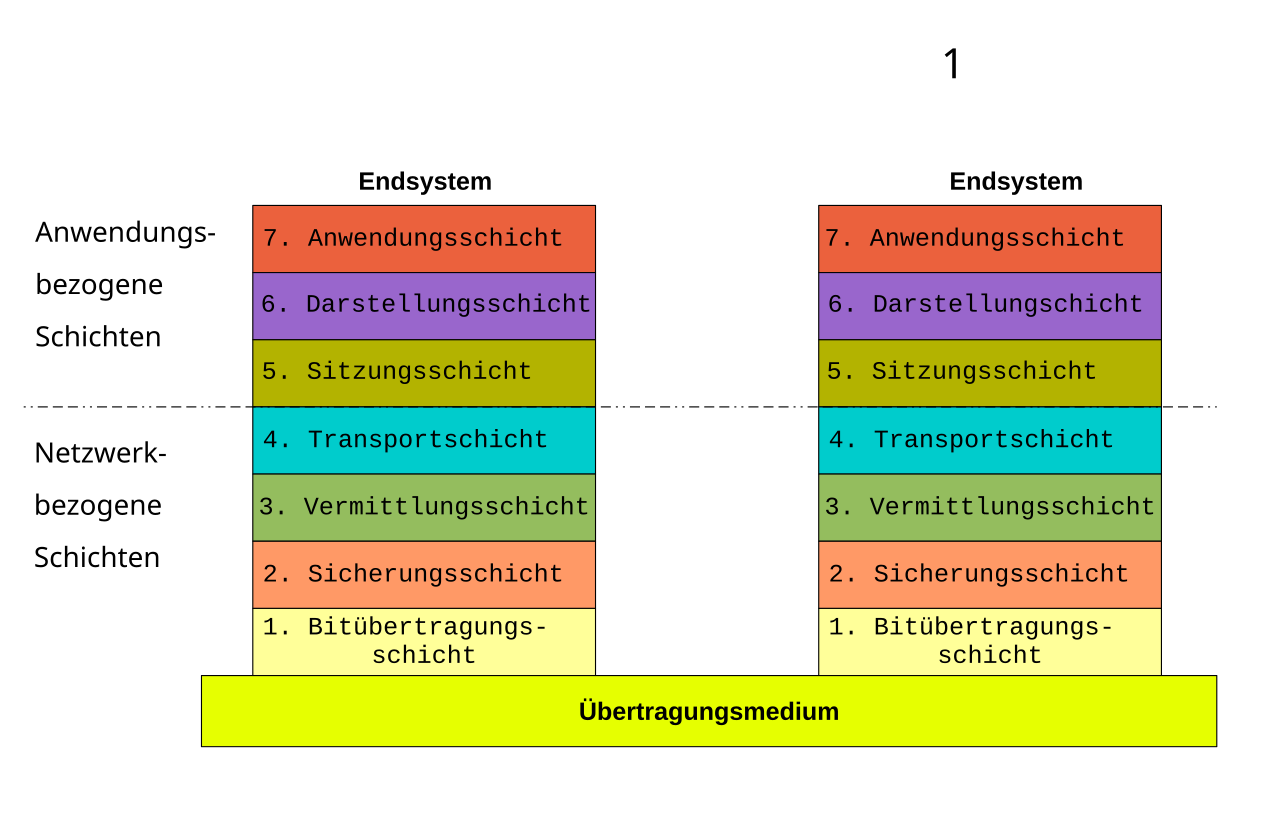
\includegraphics[width=0.75\linewidth]{picture-lib/osi.png}
    \caption{OSI Model Graphik von (Michael von Brandenburg)}
    \label{fig:placeholder}
\end{figure}

Die erste Schicht (\textbf{Die Bitübertragungsschicht}) ist die physische Schicht. Sie umfasst Antennen, Kabel, Hubs und ähnliche Hardware und dient als Medium, über das ein Bitstrom übertragen wird. Das geschieht über Kabel oder über elektromagnetische Wellen, wie beim WLAN.\\\\

Die zweite Schicht (\textbf{Die Sicherungsschicht}) regelt den Zugriff auf die physische Schicht. Sie sorgt für eine Datenflusskontrolle und dafür, dass alle Daten fehlerfrei übertragen werden. Sie besteht aus den zwei Unterschichten MAC (Media Access Control) und LLC (Logical Link Control). Die MAC-Adressen identifizieren die Hardware in einem Netzwerk. Typische Geräte dieser Schicht sind Bridges und Switches.\\\\

Die dritte Schicht (\textbf{Die Vermittlungsschicht}) vermittelt Datenpakete durch das ganze Netzwerk. Zu ihren Aufgaben gehören das Routing, also die Suche nach dem besten Weg zum Empfänger, und die Stauvermeidung bei hohem Netzwerkverkehr. Sie spielt vor allem bei Routern eine Rolle und versieht jedes Paket mit einer IP-Adresse, damit es beim richtigen Empfänger ankommt.\\\\

Die vierte Schicht (\textbf{Die Transportschicht}) sorgt dafür, dass die Datenpakete in der richtigen Reihenfolge beim Empfänger ankommen. Je nach Protokoll prüft sie auch, ob alle Pakete angekommen sind. Ausserdem weist sie den Paketen einen Port zu.\\\\

Die fünfte Schicht (\textbf{Die Sitzungsschicht}) baut eine Sitzung auf, behebt Probleme während der Sitzung und beendet sie wieder.\\\\

Die sechste Schicht (\textbf{Die Darstellungsschicht}) arbeitet wie ein Übersetzer zwischen den Daten der Anwendung und den Daten, die über das Netzwerk gehen. Sie kann Daten ausserdem komprimieren und verschlüsseln. Typische Beispiele sind UTF-8 für die Zeichenkodierung und AES für die Verschlüsselung.\\\\

Die siebte Schicht (\textbf{Die Anwendungsschicht}) verbindet den Benutzer mit den unteren Schichten. Beispiele sind Messaging-Apps und Browser. Sie nimmt die Daten des Benutzers entgegen und gibt sie an die unteren Schichten weiter.

\subsection{IP}

Das \textbf{IP} (Internet Protocol) ist eine der Grundlagen des Internets. Es gibt zwei Standards, den älteren IPv4 und den neueren IPv6, und sie unterscheiden sich im Adressraum. IPv4 erlaubt nur 2\textsuperscript{32} (4 294 967 296) Adressen, IPv6 dagegen 2\textsuperscript{128}. Das sind so viele, dass man nie erleben wird, dass sie aufgebraucht sind. Eine IP-Adresse kann man sich wie die Adresse eines Gebäudes vorstellen. Jedes Gebäude hat eine eindeutige Adresse, und genauso hat ein Router eine eindeutige öffentliche Adresse. IPv4 musste ersetzt werden, weil es nicht mehr genügend eindeutige Adressen gab. IPv6 bringt zudem Verbesserungen bei der Sicherheit.\\\\


Jedes Datenpaket, das über das Netzwerk verschickt wird, braucht eine Adresse, sonst findet es seinen Empfänger nicht. Ausserdem möchte man nicht der ganzen Welt mitteilen, was man gestern gefrühstückt hat.

\subsection{TCP}

Das \textbf{TCP} (Transmission Control Protocol) bildet zusammen mit dem IP das TCP/IP-Protokoll, das heute überall als Standard verwendet wird. Beim Netzwerk-Engineering benutzt man oft das OSI-Modell, in der Praxis läuft aber TCP/IP. Wie in Abbildung (...) zu sehen ist, findet man die meisten Elemente des OSI-Modells wieder, nur die fünfte und die sechste Schicht fehlen. Ihre Aufgaben übernimmt im TCP/IP-Modell die Anwendungsschicht. Trotzdem spricht man im Sprachgebrauch weiterhin von sieben Schichten. TCP ist ein zuverlässiges Protokoll der vierten Schicht und stellt sicher, dass alle Datenpakete richtig ankommen. Dafür verwendet es einen Three-Way-Handshake, eine Sequenzierung und eine Checksumme.

\subsection{UDP}

Das \textbf{UDP} (User Datagram Protocol) ist ebenfalls ein Protokoll der vierten Schicht. Es ist weniger zuverlässig als TCP, wird aber dort eingesetzt, wo ein schneller Datenaustausch wichtiger ist als ein kleiner Datenverlust, zum Beispiel beim DNS (Domain Name System) oder bei Anrufen.

\section{Multithreading}

\subsection{Thread}

Ein \textbf{Thread} (Ausführungsstrang) ist ein Programmablauf. Braucht ein Programm mehr als einen Thread, spricht man von Multithreading. Mit mehreren Threads lassen sich Aufgaben parallel berechnen, sodass nicht jede Funktion auf die vorherige warten muss. Als Beispiel kann man ein Programm nehmen, das Kunden bedient. Mit nur einem Thread kann es nur einen Kunden aufs Mal bedienen. Mit zwei oder mehr Threads können mehrere Kunden gleichzeitig bedient werden, ohne dass sie auf den Kunden vor ihnen warten müssen.

\subsection{Daemon Thread}

in \textbf{Daemon Thread} ist ein Thread, der im Hintergrund läuft. Das Programm wartet nicht darauf, dass er fertig wird, und er endet automatisch, sobald alle normalen Threads beendet sind. Der Begriff leitet sich von Hintergrunddiensten (Daemons) ab.

\section{Verschlüsselung}

\subsection{Allgemeine Bedeutung}

\textit{"Bei der Verschlüsselung wird lesbarer Klartext in unlesbaren Chiffretext umgewandelt, um sensible Informationen vor unbefugten Benutzern zu verbergen. Unternehmen nutzen regelmäßig Verschlüsselung im Bereich Datensicherheit, um sensible Daten vor unberechtigtem Zugriff und Data Breaches zu schützen."}\citep{ai-wikipedia}\todo{Ändere die Quelle IBM Verschlüsselung}\\
Die \textbf{Verschlüsselung} gibt es schon seit mehreren tausend Jahren. Aus dem Altertum sind viele verschlüsselte Nachrichten dokumentiert. Die Methoden haben sich stetig weiterentwickelt, bis zu den heutigen Verfahren, die auch ein herkömmlicher Computer ohne den Schlüssel nicht entziffern kann. Der Grund dafür ist, wie das Zitat zeigt, der Schutz privater Daten vor unbefugten Personen. Im Netzwerk sind viele sogenannte "Black Hat"-Hacker unterwegs, die Daten stehlen und für hohe Summen zurück- oder weiterverkaufen. Würde man Daten nicht jederzeit verschlüsseln, würde man ihnen diese auf dem Silbertablett servieren.

\subsection{XOR}

Das \textbf{XOR-Gatter} (Exklusiv-Oder-Gatter) ist eine Schaltung, die ein Signal nur weiterleitet, wenn die beiden Eingangssignale verschieden sind. Sind sie gleich, gibt sie kein Signal weiter.

\[Y=A\veebar B\]
Mit XOR kann man auch Bits verschlüsseln. Das Verfahren allein ist aber leicht zu brechen, weil sich wiederholende Muster im Schlüssel eine Schwachstelle sind. Trotzdem bauen viele Verschlüsselungsverfahren auf XOR auf. Ein Bit hat nur zwei Zustände, wahr (1) oder falsch (0), und um diese zu verknüpfen, braucht es eine Schaltung wie das XOR.

\subsection{Advanced Encryption Standard (AES)}

Der \textbf{Advanced Encryption Standard} ist ein symmetrischer Verschlüsselungsalgorithmus, der in vier Operationen arbeitet, die in mehreren Runden wiederholt werden. Er gilt als Verschlüsselungsstandard, weil es nach heutigem wissenschaftlichem Stand keine Methode gibt, die Verschlüsselung zu brechen, ausser man besitzt den Schlüssel oder es passiert ein Fehler im Prozess selbst. Der Grund liegt im Aufbau des Algorithmus, der mit einer 4x4-Matrix arbeitet. Jede Zelle dieser Matrix enthält 1 Byte (8 Bit), insgesamt sind es also 16 Bytes (128 Bit). Der Schlüssel kann bei AES 128, 192 oder 256 Bit lang sein.\\\\
Zuerst wird eine \textbf{Substitutionsbox} (S-Box) konstruiert, mit der in der ersten Operation jedes Byte ersetzt werden kann. Mathematisch wird sie wie folgt berechnet:\\\\
\(\mathbb{F}_{2^8}\) ist ein endlicher Körper. Mit der Funktion \(S(x)\) wird für jedes Byte eine inverse und eine affine Transformation berechnet.
\[S(x)=\bar{x}\oplus(\bar{x}\lll1)\oplus(\bar{x}\lll2)\oplus(\bar{x}\lll3)\oplus(\bar{x}\lll4)\oplus(63)\small{hex}\]
\(\bar{x}\) ist die multiplikative Inverse von \(x\) in \(\mathbb{F}_{2^8}\). \(b\lll n\) ist die Linksrotation der Bits um \(n\) Positionen. \(\oplus\) ist die XOR-Verknüpfung.\\\\
Als Nächstes nimmt der Algorithmus den Schlüssel und erzeugt daraus \(R +1\) Teilschlüssel, von denen jeder in einer Runde verwendet wird. Insgesamt werden \(b\cdot(R+1)\) Bit benötigt, wobei \(b\) die Blockgrösse ist.\\\\
Für \(i=N,\dots,b/32\cdot(R+1)-1:\)
\[W_i=\left\{ \begin{array}{@{}lcl@{}}
W_{i-N}\oplus S(W_{i-1}\lll8)\oplus C_{i/N-1} & \mbox{wenn} & i \equiv 0 \mbox{ (mod } N)\\ W_{i-N}\oplus S(W_{i-1}) & \mbox{wenn} & N>6 \mbox{ und } \equiv 4 \mbox{ (mod }N)\\
W_{i-N}\oplus W_{i-1} & \mbox{sonst}
\end{array}\right.\]
Diese Formel beschreibt die \textbf{Schlüsselexpansion}, bei der der ursprüngliche Schlüssel erweitert wird, ohne dass ein leicht erkennbares Muster entsteht. Der Schlüssel wird zuerst in die Wörter \(W_0,\dots,W_{N-1}\) aufgeteilt und dann mithilfe von \(W_i\) erweitert. \(S(x)\) ist die S-Box-Funktion und sorgt für die Durchmischung. Für \(C_j\) berechnet man \(2^j\) im Körper \(\mathbb{F}_{2^8}\) und setzt das Ergebnis in das höchste Byte der Konstante \(C_j\) ein. In der Graphik (\todo{graphik}) ist das besser zu erkennen.\\\\
Die berechneten Rundenschlüssel werden in der vierten Operation (AddRoundKey) zur Matrix addiert. Die erste Operation ist \textbf{SubBytes}, bei der jedes Byte der Matrix in \(S(x)\) eingesetzt wird.\\ Danach folgt \textbf{ShiftRows}, bei dem die Zeilen der Matrix verschoben werden. Die erste Zeile bleibt unverändert, die zweite wird um eine Position verschoben, die dritte um zwei und die vierte um drei.\\ Dann folgt \textbf{MixColumns}, das die Spalten vermischt. Um das Byte \(b_j\) zu berechnen, wird jedes \(a_j\) der alten Spalte mit den Konstanten 1, 2 oder 3 multipliziert.

\begin{align}
b_0 = (a_0\cdot2)\oplus(a_1\cdot3)\oplus(a_2\cdot1)\oplus(a_3\cdot1)\\
b_1 = (a_0\cdot1)\oplus(a_1\cdot2)\oplus(a_2\cdot3)\oplus(a_3\cdot1)\\
b_2 = (a_0\cdot1)\oplus(a_1\cdot1)\oplus(a_2\cdot2)\oplus(a_3\cdot3)\\
b_3 = (a_0\cdot3)\oplus(a_1\cdot1)\oplus(a_2\cdot1)\oplus(a_3\cdot2)\\
\end{align}

Matrix:
\[\begin{pmatrix}
b_0\\ b_1\\ b_2\\ b_3 \\ 
\end{pmatrix}=
\begin{pmatrix}
2 & 3 & 1 & 1\\ 
1 & 2 & 3 & 1\\ 
1 & 1 & 2 & 3\\  
3 & 1 & 1 & 2 
\end{pmatrix}\begin{pmatrix}
a_0\\ a_1\\ a_2\\ a_3 \\ 
\end{pmatrix}\]
Im Galois-Körper \(GF(2^8)\) gilt:

\begin{align}
&a\cdot1=a\\
&a\cdot2=\left\{ \begin{array}{@{}lcl@{}}
2a & \mbox{wenn} & a < 2^7\\
2a\oplus(11b)\small{hex} & \mbox{wenn} & a \geq 2^7\\
\end{array}\right.\\
&a\cdot3=(a\cdot2)\oplus a
\end{align}


Die letzte Operation ist AddRoundKey. Sie verknüpft den Rundenschlüssel per XOR mit der Matrix und beendet damit einen Durchgang der Schleife. Dieser wird je nach Schlüssellänge 10, 12 oder 14 Mal wiederholt: Je länger der Schlüssel, desto mehr Runden werden benötigt. Die Entschlüsselung läuft genau umgekehrt ab.

\section{Datenpakete}

\subsection{Aufbau}

Der Aufbau eines \textbf{Datenpakets} hängt vom Protokoll ab. Man könnte auch ein eigenes Protokoll verwenden, aber kein anderes Gerät könnte es lesen, weil überall das Standardprotokoll TCP/IP verwendet wird. Dieses folgt der OSI-Struktur ohne die Sitzungs- und die Darstellungsschicht. Das Datenpaket wird zuerst in der Anwendungsschicht aufgebaut. Als Beispiel nehme ich den Verbindungsaufbau zu einer Webseite. In der Anwendungsschicht wird HTTPS festgelegt, entweder weil der Benutzer den Link selbst eingegeben hat oder weil das DNS die richtige Seite gefunden hat. Das erste Stück besteht aus dem HTTPS-Teil und den Daten, die an die nächste Schicht weitergegeben werden. In der Transportschicht kommt ein L4-Header (Layer 4) dazu, der festlegt, ob TCP oder UDP verwendet wird, und der die Portnummer enthält. In der Vermittlungsschicht wird der L3-Header hinzugefügt, der die Source-IP und die Destination-IP enthält. In der Sicherungsschicht wird das Paket von einem L2-Header und einem L2-Trailer umhüllt und wird so zu einem Frame. Dieser enthält die MAC-Adressen von Sender und Empfänger. Zum Schluss wird das Paket über die Bitübertragungsschicht verschickt, bis es beim Zielgerät ankommt, in diesem Fall beim Server der Webseite.

\subsection{Translation}

Datenpakete enthalten alle diese Informationen als Bytes. Computer können sie leicht lesen, für Menschen sind sie aber unbrauchbar. Ausserdem sind Nachrichten meist verschlüsselt. Darum braucht es die Darstellungsschicht, die den Binärcode in Zeichen umwandelt. Das geschieht mit ASCII oder UTF-8, wobei jede Bitkombination einem Zeichen zugeordnet wird. Die Ver- und Entschlüsselung findet vor beziehungsweise nach dieser Übersetzung statt.

\chapter{Konzeption und Methodik}
\label{chap:Konzeption und Methodik}

\section{Python}

Python ist eine weitverbreitete Programmiersprache, die von der Python Software Foundation weiterentwickelt wird. Ihr Designer ist Guido van Rossum. Die Sprache wurde in den 90er-Jahren entwickelt und hätte ursprünglich als Skriptsprache für das Betriebssystem Amoeba gedient. 1994 erschien Python 1.0. Die aktuellste Version ist 3.14.8. Python eignet sich für Anfänger und für Experten, weil die Sprache leicht verständlich ist und viele Libraries (Bibliotheken) hat, aber auch komplexe Aufgaben lösen kann. In Python ist jeder Datentyp ein Objekt.

\section{Libraries}

\subsection{Socket}

Socket ist eine Bibliothek, welche Verbindungen erstellt mit Server und Client. Sockets kommen ursprünglich aus dem ARPANET (Advanced Research Projects Agency Network), wo schon seit 1971 benutzt wurden. Sockets arbeiten mit dem TCP/IP, weswegen sie eine zuverlässige Verbindung zischen mehreren Geräten erzeugen können. Das Socket übernimmt alle tiefen Schichten des OSI-Models, von der Sicherungsschich bis hin zur Sitzungsschicht.

\subsection{Threading}

Threading ist eine Bibliothek, welche erlaubt mehrere Operationen Scheinweise parallel zu bearbeiten. Es ermöglicht Prozesse die einen Stau bei der Ausführung verursachen könnten zu verhindern. Indem es diese als separate Operationen aufteilt.

\subsection{Tkinter}

Tkinter ist eine Bibliothek, welche eine ressourcenschonendes GUI (graphical user interface) erstellt, die vollkommen selbst gestaltbar ist. Mit dieser kann man Fenster bauen, die alle benötigten Nutzereingaben nehmen und weiterleiten können. Im OSI-Model wäre sie die Anwendungsschicht. Es gibt auch eine erweiterte Bibliotheken, die Tkinter als Fundament verwendet, aber zusätzlich die GUI attraktiver gestalten. Beispielsweise das CustomTkinter, welches in dieser Arbeit verwendet wird.

\subsection{Pycryptodomex}

Pycryptodomex ist eine Bibliothek, welche eine Vielzahl an modernen Verschlüsselungen beinhaltet. Sie ist aber ein Fork vom alten Pycryptodome, weil es oft zu Bibliothekkonflikten mit dem original kommt. Diese Bibliothek beinhaltet alle Algorithmen, welche für jede Verschlüsselung benötigt wird.

\chapter{Umsetzung und Ergebnisse}
\label{chap:Umsetzung und Ergebnisse}
\section{Umsetzung}
\subsection{Einfache Echo-Nachricht}
Das Projekt begann ich mit der Datei \texttt{main.py}, die später zur Server-Datei wurde (siehe unten). Ihre Aufgabe bestand zunächst darin, sich mit einem Client zu verbinden und empfangene Nachrichten unverändert zurückzusenden. Dazu wird ein Socket an die IP-Adresse des Servers und den festgelegten Port 7367 gebunden. Mit \texttt{server.listen()} wartet der Socket auf Verbindungsanfragen, und \texttt{server.accept()} nimmt eine Anfrage an. Der zugrunde liegende Three-Way-Handshake wird dabei vom Betriebssystem durchgeführt. Mit \texttt{client.recv(1024)} empfängt der Server die Daten des Clients und sendet sie mit \texttt{client.sendall(data)} zurück. Die Methode \texttt{sendall()} wiederholt den Sendevorgang, bis alle Bytes übertragen sind. Bei \texttt{send()} kann es dagegen vorkommen, dass nur ein Teil der Daten gesendet wird.\\

\begin{figure}[H]
    \centering
    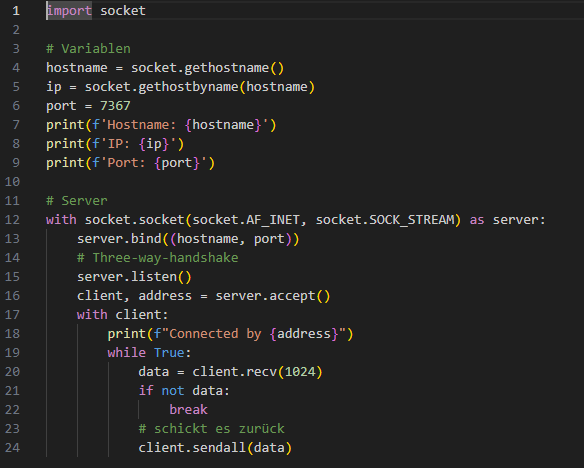
\includegraphics[width=0.5\linewidth]{picture-lib/Screenshot 2026-10-07 020521.png}
    \caption{Server.py V1}
    \label{fig:A0}
\end{figure}

Danach erstellte ich die Datei \texttt{client.py}, die der Benutzer benötigt, um mit dem Server zu kommunizieren. Sie verbindet sich mit der IP-Adresse des Servers und dem Port 7367 und sendet die Nachricht "Test" als Bytes. Anschliessend wartet sie auf die Antwort des Servers und wandelt die empfangenen Bytes wieder in eine Zeichenkette (String) um.\\

\begin{figure}[H]
    \centering
    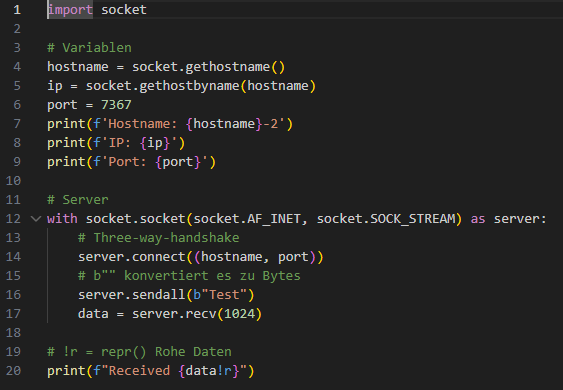
\includegraphics[width=0.5\linewidth]{picture-lib/Screenshot 2026-10-07 020618.png}
    \caption{Client.py V1}
    \label{fig:A1}
\end{figure}

Mit diesen beiden Dateien war ein erster Nachrichtenaustausch zwischen Server und Client möglich.

\subsection{Mehrere Benutzer}

Als Nächstes erweiterte ich den Server so, dass mehrere Clients gleichzeitig kommunizieren können, ohne aufeinander warten zu müssen. Der Server bindet sich wie zuvor an IP-Adresse und Port. Mit \texttt{server.listen(5)} legt er jedoch eine Warteschlange von höchstens fünf unbearbeiteten Verbindungsanfragen fest. Danach läuft eine while-Schleife, die jede eingehende Verbindung annimmt. Mit der Bibliothek Threading wird für jeden Client ein eigener Thread erstellt, der die Funktion \texttt{client\_handler(client)} ausführt. Innerhalb dieser Funktion läuft eine weitere while-Schleife, die auf eingehende Daten wartet. Sie wird beendet, wenn der Client die Verbindung trennt oder ein Fehler auftritt. Andernfalls sendet der Server die Daten in umgekehrter Reihenfolge zurück (\texttt{data[::-1]}).

\begin{figure}[H]
    \centering
    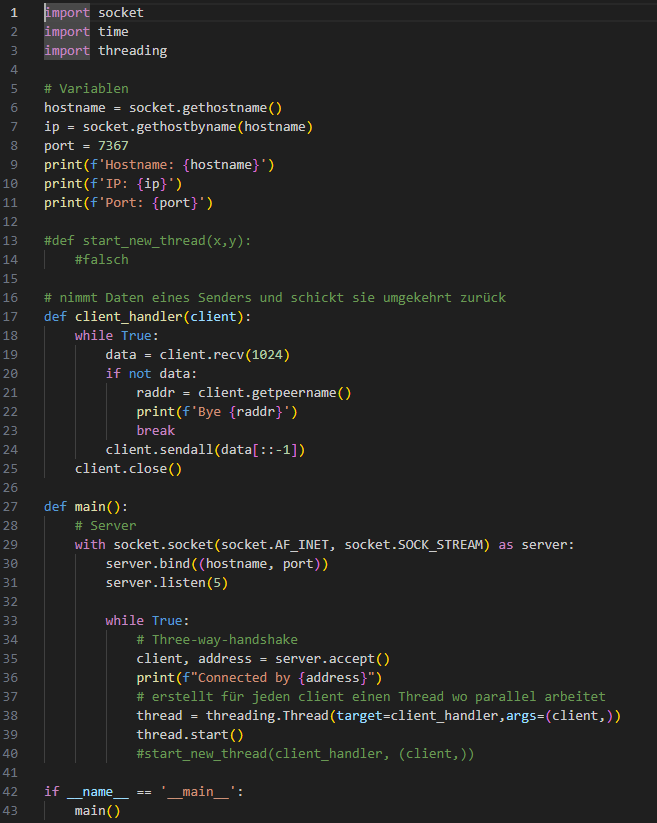
\includegraphics[width=0.5\linewidth]{picture-lib/Screenshot 2026-10-07 022627.png}
    \caption{Server.py V2}
    \label{fig:A2}
\end{figure}

Auch die Client-Datei wurde überarbeitet. Eine while-Schleife ermöglicht nun mehrere Nachrichten nacheinander. Zudem liest das Programm die Eingabe im Terminal mit \texttt{input()} und speichert sie in der Variable \texttt{message}. Diese wird mit der Zeichenkodierung ASCII in Bytes umgewandelt und gesendet. Die Antwort des Servers wird anschliessend mit ASCII dekodiert und dem Benutzer angezeigt. Am Ende jedes Durchlaufs fragt das Programm, ob der Benutzer fortfahren möchte. Bei der Eingabe "y" beginnt die Schleife von vorn, bei jeder anderen Eingabe wird die Verbindung getrennt.

\begin{figure}[H]
    \centering
    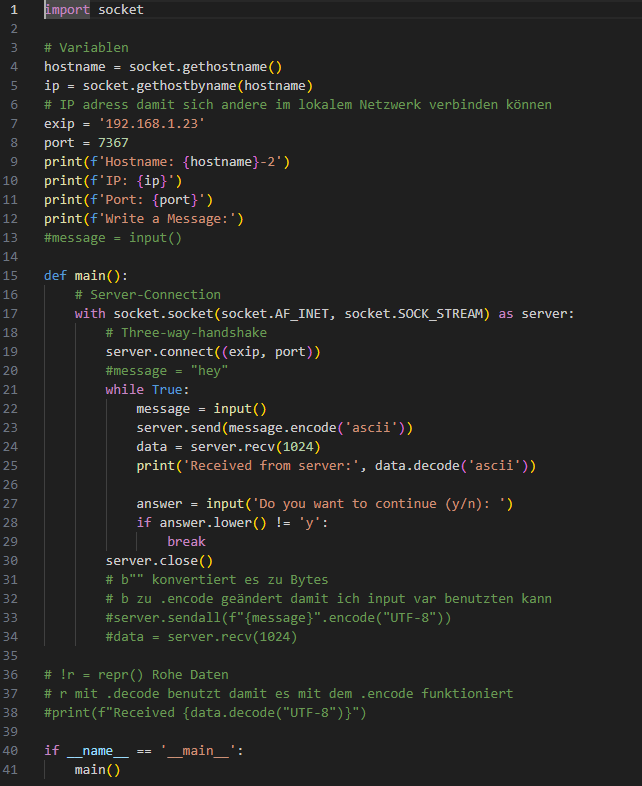
\includegraphics[width=0.5\linewidth]{picture-lib/Screenshot 2026-10-07 022613.png}
    \caption{Client.py V2}
    \label{fig:A3}
\end{figure}

Beide Dateien zusammen erlauben den Datenaustausch zwischen mehreren Clients und dem Server. Die Clients können in dieser Version nur mit dem Server Daten austauschen, untereinander ist keine Kommunikation möglich.

\subsection{Austausch von Informationen}

In der nächsten Version wurde die Kommunikation zwischen Benutzern ermöglicht. Der Server empfängt eine Nachricht von einem Client und leitet sie an den richtigen Empfänger weiter. Der Verbindungsaufbau blieb bis auf eine Ausnahme gleich: Es wird nun eine Liste \texttt{client\_connections} geführt, in die jeder verbundene Client eingetragen wird. Diese Liste wird an den \texttt{client\_handler} übergeben. Er wartet innerhalb eines \texttt{try}-Blocks auf Daten. Treten Fehler auf, bricht er den Vorgang ab, sendet eine Fehlermeldung, schliesst die Verbindung und entfernt den Client aus der Liste.
Treffen Daten ein, wird zwischen einer Nachricht und dem Befehl \texttt{GET\_LIST} unterschieden. Bei diesem Befehl sendet der Server dem Client die Liste aller aktuell verbundenen Clients, ohne den Anfragenden selbst. Das wird mit der Bedingung \texttt{if x != address} geprüft. Die übrigen Adressen werden in der Variable \texttt{users} gespeichert, mit \texttt{.join(users)} zu einer Zeichenkette verbunden, mit ASCII kodiert und gesendet.
Handelt es sich um eine Nachricht, prüft der Server zuerst die IP-Adresse des Empfängers mithilfe der Statusvariable \texttt{found} (Flag). Eine Schleife vergleicht dazu alle bestehenden Verbindungen mit der Empfängeradresse. Bei einer Übereinstimmung wird die Nachricht gesendet, \texttt{found} auf wahr gesetzt und die Schleife beendet. Existiert der Empfänger nicht oder ist er nicht mehr verbunden, bleibt \texttt{found} falsch, und \texttt{if not found:} meldet dem Absender, dass der Empfänger nicht gefunden wurde.

\begin{figure}[H]
    \centering
    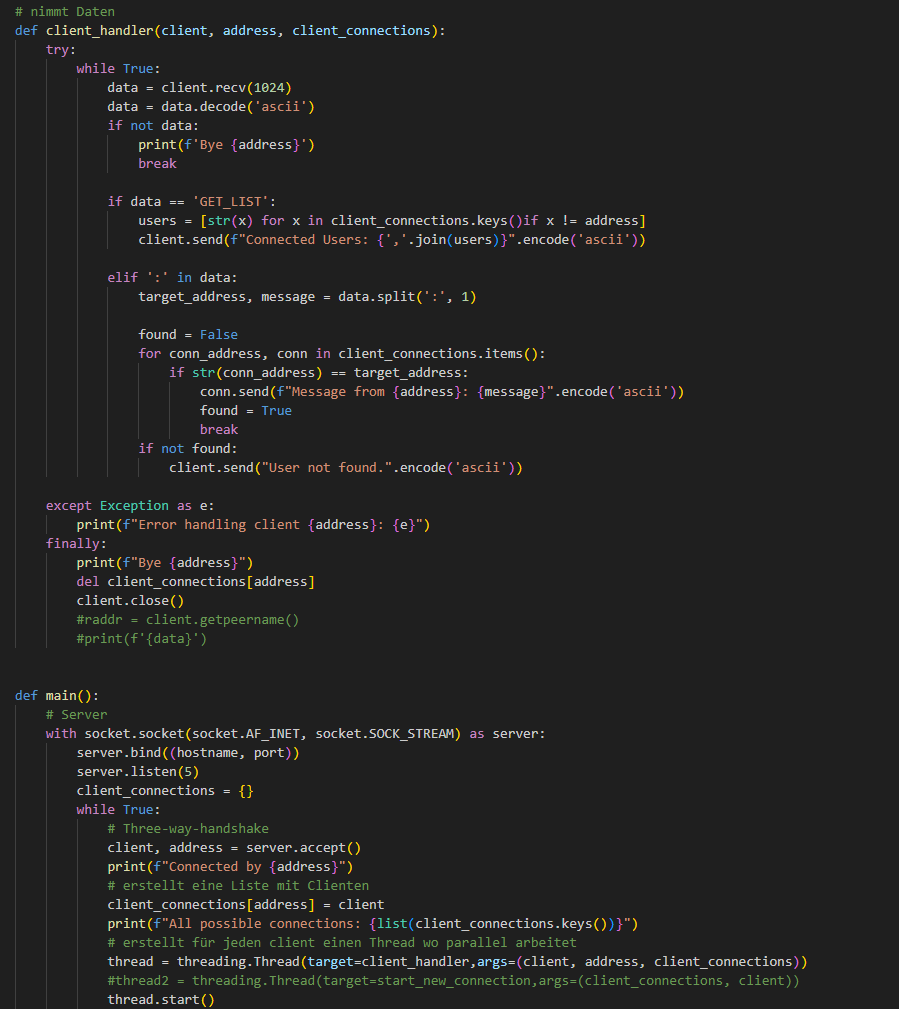
\includegraphics[width=0.5\linewidth]{picture-lib/Screenshot 2026-10-07 025514.png}
    \caption{Server.py V3}
    \label{fig:A4}
\end{figure}

In der Client-Datei wurde ein Daemon Thread ergänzt, damit die Eingabe des Benutzers nicht blockiert wird. Dieser führt die Funktion \texttt{receive\_messages(client\_data)} aus, die in einer Schleife auf Nachrichten wartet. Durch den Wert \texttt{daemon=True} läuft sie im Hintergrund, übersetzt alle ankommenden Daten mit ASCII und zeigt sie im Terminal an. Gleichzeitig läuft eine Schleife für die Eingabe, die bei jedem Durchlauf drei Fälle unterscheidet. Gibt der Benutzer \texttt{list} ein, sendet der Client den Befehl \texttt{GET\_LIST} an den Server. Bei \texttt{exit} wird die Schleife beendet. Jede andere Eingabe wird als Nachricht an den Server gesendet. In dieser Version muss der Benutzer IP-Adresse, Port und Nachricht selbst eingeben. Bei einer fehlerhaften Eingabe kommt die Nachricht nicht beim gewünschten Empfänger an.

\begin{figure}[H]
    \centering
    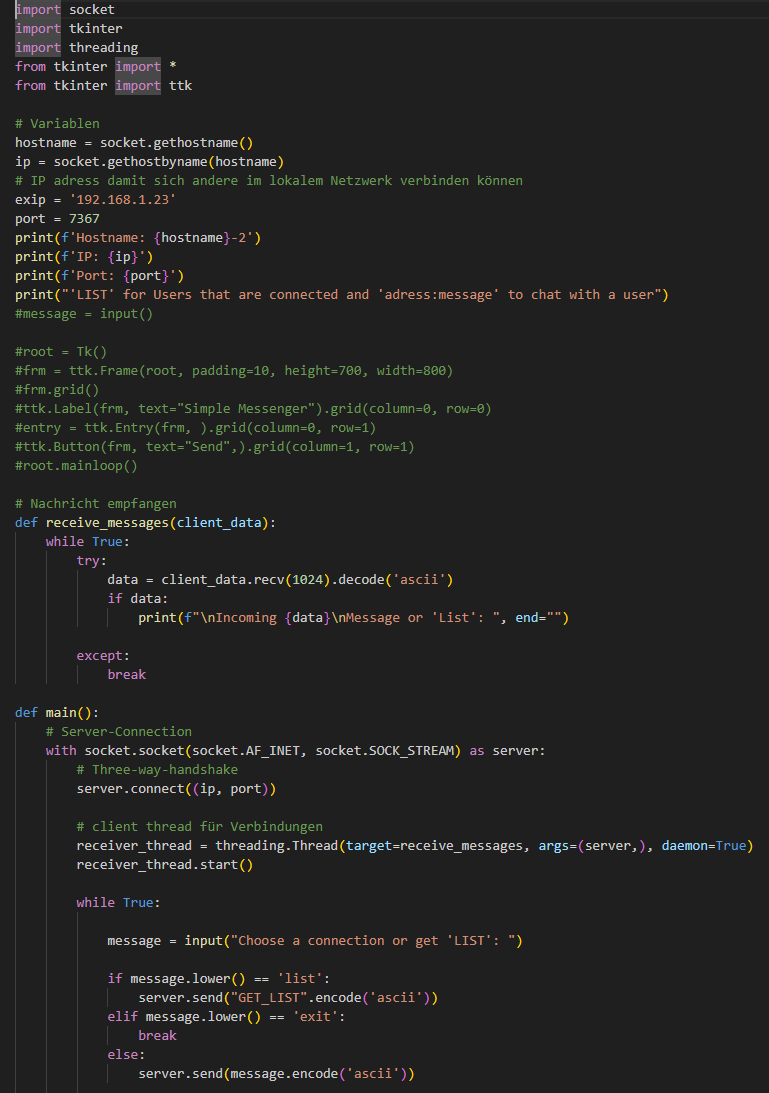
\includegraphics[width=0.5\linewidth]{picture-lib/Screenshot 2026-10-07 025429.png}
    \caption{Client.py V3}
    \label{fig:A5}
\end{figure}

Die beiden Dateien bilden ein Backend für die Kommunikation zwischen Benutzern, das allerdings wenig benutzerfreundlich ist. Der Server speichert die Adressen der Clients, filtert sie und leitet Nachrichten an den richtigen Empfänger weiter.

\subsection{GUI für Benutzer}

Bei der Programmierung der GUI blieb die Server-Datei fast unverändert und wird hier nicht weiter behandelt. Mit der Bibliothek Tkinter lässt sich ein Frontend, also eine grafische Benutzeroberfläche, erzeugen. Zuerst mussten empfangene Nachrichten im Fenster dargestellt werden. Das funktioniert nach demselben Prinzip wie in Version 3: Die Daten werden mit ASCII dekodiert, und wie in der Server-Datei wird zwischen Liste und Nachricht unterschieden. Das Unterscheidungsmerkmal für eine Nachricht ist der Doppelpunkt. Sie wird als \texttt{notification} gespeichert und im Fenster \texttt{chat\_box} angezeigt. Enthalten die Daten keinen Doppelpunkt, werden sie als Liste behandelt. Dabei werden die Klammern jeder Adresse entfernt, die Adressen in der Liste \texttt{user\_list} gespeichert und anschliessend als Werte der Combobox hinzugefügt.

\begin{figure}[H]
    \centering
    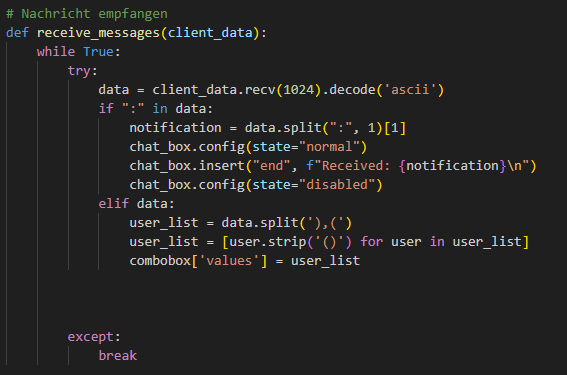
\includegraphics[width=0.5\linewidth]{picture-lib/Screenshot 2026-10-07 042912.png}
    \caption{Client.py V4 Abschnitt 1}
    \label{fig:A6}
\end{figure}

In der Hauptfunktion wird die GUI aufgebaut. Zuerst entsteht mit \texttt{tk.Tk()} das Fenster, das alle Widgets enthält. Anschliessend werden die Widgets Label, Text, Button, Combobox und Entry erstellt und in Variablen gespeichert. Wichtig sind die beiden Schaltflächen und das Eingabefeld. Die Schaltfläche "Get List" (\texttt{button2}) ruft die Funktion \texttt{get\_list()} auf, die dem Server den Befehl \texttt{GET\_LIST} sendet. Die Schaltfläche "Send" ruft die Funktion \texttt{send()} auf.

\begin{figure}[H]
    \centering
    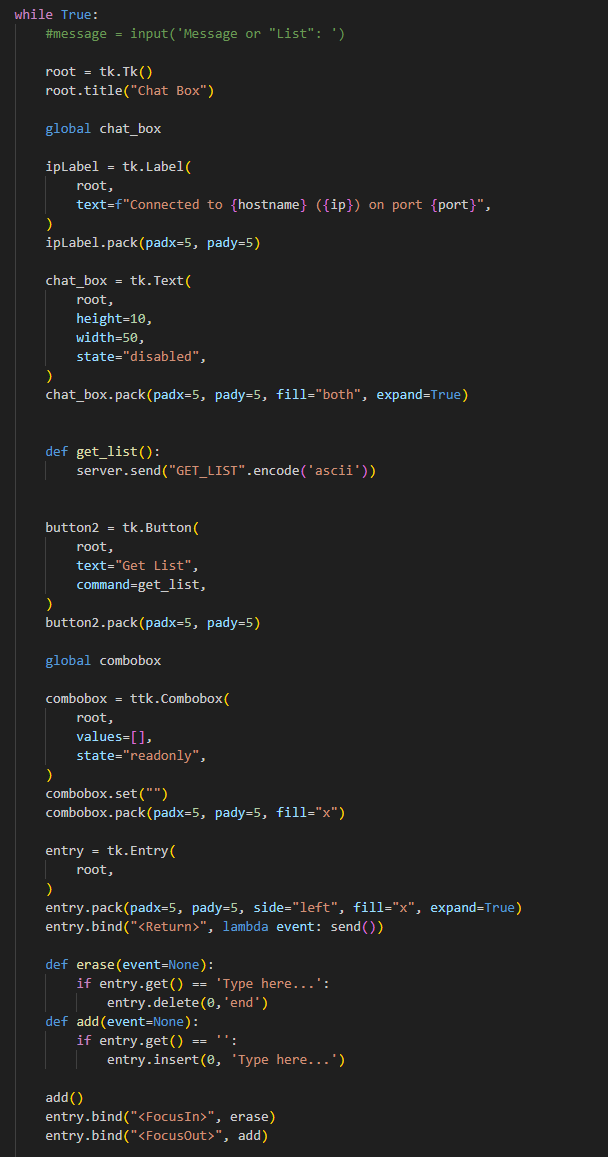
\includegraphics[width=0.45\linewidth]{picture-lib/Screenshot 2026-10-07 042949.png}
    \caption{Client.py V4 Abschnitt 2}
    \label{fig:A7}
\end{figure}

Die Funktion \texttt{send()} übernimmt mehrere Aufgaben. Zuerst liest sie die vom Benutzer in der Combobox ausgewählte Adresse und kombiniert sie mit dem Text aus dem Eingabefeld zur Variable \texttt{message}. Danach sendet sie die Nachricht an den Server und zeigt im Chatverlauf an, welche Nachricht an wen gesendet wurde. Anschliessend leert sie das Eingabefeld und verändert den Fensterfokus, damit der Platzhalter "Type here\dots" wieder erscheint. Beim Schreiben verschwindet er erneut. Beim Schliessen des Fensters erscheint eine Sicherheitsabfrage. Bestätigt der Benutzer mit "Yes", werden das Fenster und die Verbindung geschlossen, damit das Programm nicht im Hintergrund weiterläuft.

\begin{figure}[H]
    \centering
    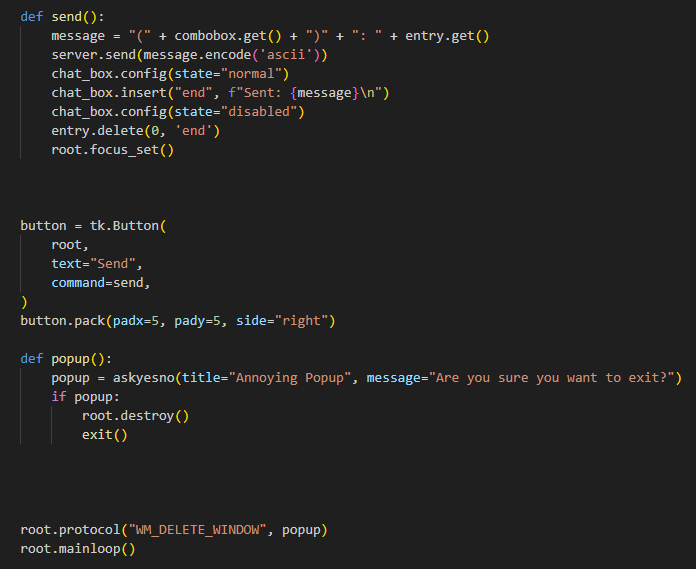
\includegraphics[width=0.5\linewidth]{picture-lib/Screenshot 2026-10-07 043004.png}
    \caption{Client.py V4 Abschnitt 3}
    \label{fig:A8}
\end{figure}

Daraus ergibt sich die Chat Box in der Abbildung \ref{fig:A9}.

\begin{figure}[H]
    \centering
    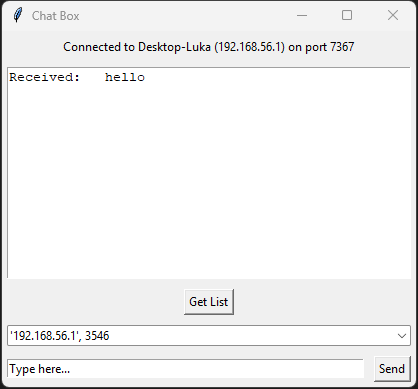
\includegraphics[width=0.5\linewidth]{picture-lib/Screenshot 2026-10-07 045701.png}
    \caption{Chat Box}
    \label{fig:A9}
\end{figure}

Über diese Oberfläche kann der Benutzer einen aktuell mit dem Server verbundenen Teilnehmer auswählen und ihm Nachrichten senden sowie selbst Nachrichten empfangen. Alle Nachrichten erscheinen im Chatverlauf.

\subsection{Verschlüsselung und separates Protokoll}

In der separaten Datei \texttt{test.py} experimentierte ich, bis ich die Verschlüsselung verstanden hatte, und entwickelte ein eigenes Protokoll, das innerhalb des bestehenden Socket-Protokolls arbeitet. Die Sockets selbst lassen sich kaum verändern, und Methoden ohne Sockets werden vom Schulnetzwerk gesperrt. Deshalb kann ich nur die über die Sockets übertragenen Daten beeinflussen.
Aus der Bibliothek Pycryptodomex importierte ich AES, womit sich Bytes ver- und entschlüsseln lassen. Zuerst erstellte ich eine Beispielnachricht und wandelte sie in Bytes um. Als Testschlüssel wählte ich die 16 Byte lange Zeichenkette "Sixteen byte key", die ebenfalls in Bytes umgewandelt wird. Um den Code im eigentlichen Projekt wiederzuverwenden, definierte ich die Funktion \texttt{cipher\_message(message, key)}. Sie erhält die Nachricht als String und den Schlüssel als Bytes. Bei jedem Aufruf wird eine neue Verschlüsselung mit \texttt{AES.new(key, AES.MODE\_EAX)} im EAX-Modus (Encrypt-then-Authenticate-then-Translate) erzeugt.\citep{EAXModus2021} EAX verschlüsselt und authentifiziert die Nachricht. Wird sie auf dem Weg manipuliert, meldet der Empfänger mit dem richtigen Schlüssel dies bei der Prüfung.
Für die Verschlüsselung wird ausserdem ein Nonce (number used once) erzeugt, eine zufällige Zahl, die mit den Daten und dem Schlüssel verknüpft wird. Der Nonce darf öffentlich bekannt sein, darf sich aber bei demselben Schlüssel nie wiederholen, da sonst die Sicherheit der Verschlüsselung verloren geht. Anschliessend wird die Nachricht mit \texttt{cipher.encrypt\_and\_digest()} verschlüsselt. Innerhalb der Klammer wird der String mit UTF-8 in Bytes umgewandelt, da UTF-8 auch Sonderzeichen wie ä, ö und ü unterstützt. Zusätzlich liefert EAX einen Tag, der zur Validierung dient. Die Funktion gibt Tag, Nonce und verschlüsselten Text zurück.

\begin{figure}[H]
    \centering
    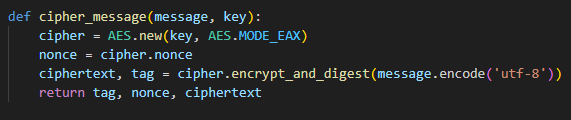
\includegraphics[width=0.75\linewidth]{picture-lib/Screenshot 2026-10-07 194013.png}
    \caption{Test.py Abschnitt 1}
    \label{fig:A10}
\end{figure}

Danach plante ich den Aufbau eines eigenen Protokolls. Ich skizzierte es zuerst auf Papier und stelle es hier als Tabelle \ref{tab:T1} dar.

\begin{table}[H]
    \centering
    \begin{tabular}{|c|c|c|c|c|c|}\hline
          Indikator&  IP&  Port&  Tag&  Nonce& Kryptogramm\\\hline
  [0x0], [0x1] oder [0x2]& 192.168.1.x& 7376& Prüfsumme& Zufällige Zahl&Vermischte Bytes\\ \hline 
    \end{tabular}
    \caption{Eigenes Protokoll}
    \label{tab:T1}
\end{table}

Anschliessend setzte ich es in der Funktion \texttt{construct\_message(\dots)} um. Sie erhält IP-Adresse, Port, Tag, Nonce und Kryptogramm und fügt sie zu einem eigenen Datenpaket zusammen. Zuerst werden IP-Adresse (String) und Port (Integer) mit der Bibliothek Socket in Bytes umgewandelt. Danach wird das Datenpaket in der Reihenfolge der Tabelle aufgebaut. Da es sich um eine Nachricht handelt, ist das erste Byte der Indikator [0x1].

\begin{figure}[H]
    \centering
    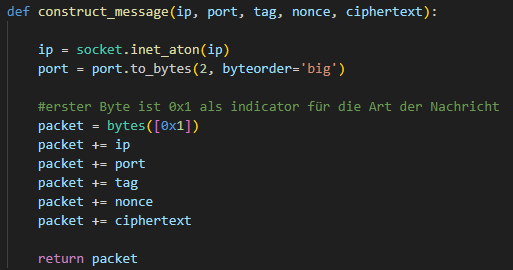
\includegraphics[width=0.5\linewidth]{picture-lib/Screenshot 2026-10-07 194028.png}
    \caption{Test.py Abschnitt 2}
    \label{fig:A11}
\end{figure}

Zuletzt definierte ich die Umkehrfunktion \texttt{decipher\_message(\dots)}. Sie benötigt denselben Schlüssel wie der Sender sowie Tag und Nonce. Mit Nonce und Schlüssel erzeugt sie dasselbe Verschlüsselungsobjekt wie der Sender. Das Kryptogramm wird mit \texttt{cipher.decrypt()} entschlüsselt und liegt danach als Klartext in Bytes vor. Mit \texttt{cipher.verify(tag)} wird die Gültigkeit geprüft. Ist sie gegeben, gibt die Funktion die Nachricht zurück, andernfalls eine Fehlermeldung.

\begin{figure}[H]
    \centering
    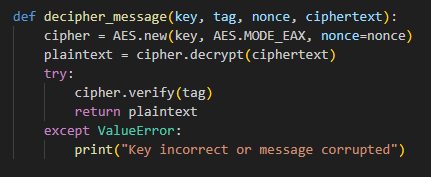
\includegraphics[width=0.5\linewidth]{picture-lib/Screenshot 2026-10-07 193959.png}
    \caption{Test.py Abschnitt 3}
    \label{fig:A12}
\end{figure}

Diese drei Funktionen ermöglichen den Austausch verschlüsselter Nachrichten in einem Netzwerk. Zudem lässt sich damit prüfen, ob die Daten auf dem Weg zum Empfänger verändert oder beschädigt wurden.

\section{Ergebnisse}

\subsection{Serverseite}

Zu Beginn werden die wichtigen Variablen des Servers festgelegt. Dazu gehört ein Puffer (Buffer) von 4 KB, was bei ASCII-Zeichen etwa 4000 Zeichen entspricht und für Textnachrichten ausreicht. Danach folgen IP-Adresse und Port. Beim Server muss die IP-Adresse 0.0.0.0 lauten, damit er auf allen Netzwerkschnittstellen Verbindungen annimmt, und der Port darf nicht bereits belegt sein. Der gewählte Port ist allerdings schon von der Swiss Exchange belegt, was bei Geräten, die diese Verbindung offen haben, zu Konflikten führen könnte.\todo{Quelle für die Port-Belegung ergänzen} Das war mir bis zu diesem Zeitpunkt nicht bekannt, da ich die Zahl zufällig gewählt und nicht überprüft hatte.

\begin{figure}[H]
    \centering
    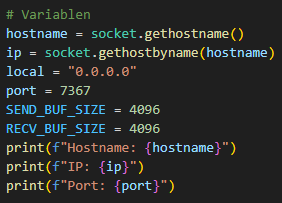
\includegraphics[width=0.5\linewidth]{picture-lib/Screenshot 2026-10-07 205017.png}
    \caption{Server.py Finale Version Abschnitt 1}
    \label{fig:A13}
\end{figure}

In der finalen Version mussten einige Funktionen angepasst werden, damit sie mit meinem Protokoll arbeiten. Der Server liest zuerst das erste Byte des Datenpakets, den Indikator, und unterscheidet damit zwischen Listenbefehl und Nachricht. Ist das erste Byte 0x0, baut er eine Liste der bestehenden Verbindungen auf, diesmal im Byte-Format. Auch diese Liste beginnt mit 0x0, damit sie als Liste erkannt wird. Für jeden Benutzer werden IP-Adresse und Port als Bytes angehängt. Das geschieht in einer for-Schleife, die alle Benutzer ausser dem anfragenden durchläuft.
Ist der Indikator 0x1, erkennt der Server eine Nachricht und liest IP-Adresse und Port des Empfängers. Stimmen sie mit einer bestehenden Verbindung überein, sendet er die Nachricht an diese Verbindung. Wird der Empfänger nicht gefunden, zeigt der Server dies an und sendet dem Absender ein Byte 0x2 als Fehlercode. Der Server liest dabei nur die ersten drei Felder des Protokolls (Indikator, IP-Adresse und Port) und hat keinen Zugriff auf den Schlüssel. Er kann den Inhalt der Nachrichten daher nie lesen, was die Privatsphäre der Benutzer schützt. Die übrigen Codeabschnitte dienen der Fehlerbehandlung auf der Serverseite.

\begin{figure}[H]
    \centering
    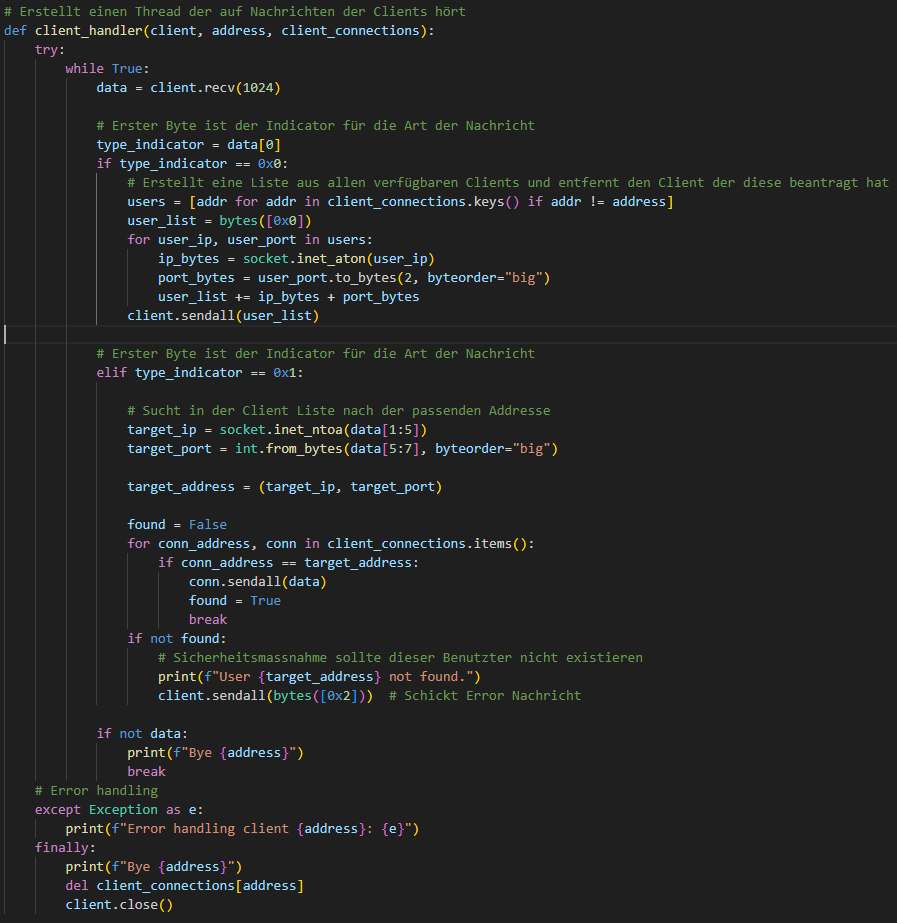
\includegraphics[width=0.6\linewidth]{picture-lib/Screenshot 2026-10-07 205030.png}
    \caption{Server.py Finale Version Abschnitt 2}
    \label{fig:A14}
\end{figure}

Beim Annehmen von Verbindungen hat sich wenig verändert. Es wurde lediglich die Puffergrösse von 4 KB ergänzt.

\begin{figure}[H]
    \centering
    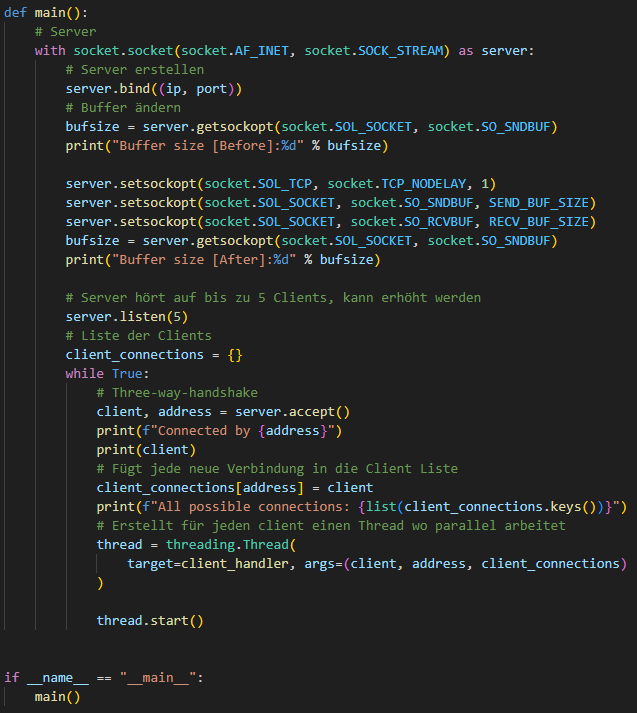
\includegraphics[width=0.5\linewidth]{picture-lib/Screenshot 2026-10-07 205047.png}
    \caption{Server.py Finale Version Abschnitt 3}
    \label{fig:A15}
\end{figure}

\subsection{Clientseite}

Hier werden Schlüssel und Variablen der Clientseite festgelegt. Wichtig ist, dass nur Benutzer mit demselben Schlüssel miteinander kommunizieren können. Der Schlüssel lässt sich jederzeit ändern, muss aber genau 16, 24 oder 32 Bytes lang sein. Ein längerer Schlüssel bietet mehr Sicherheit, verlängert aber das Ver- und Entschlüsseln leicht. Zudem müssen \texttt{exip} und \texttt{port} der IP-Adresse und dem Port des Servers entsprechen. Diese drei Werte müssen je nach Einsatz angepasst werden.

\begin{figure}[H]
    \centering
    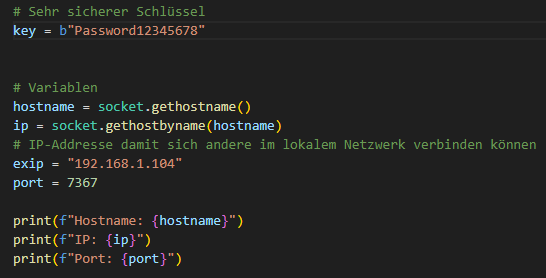
\includegraphics[width=0.5\linewidth]{picture-lib/Screenshot 2026-10-07 205128.png}
    \caption{Client.py Finale Version Abschnitt 1}
    \label{fig:A16}
\end{figure}

Die drei Funktionen aus \texttt{test.py} wurden übernommen. Zudem wurden kleinere Fehler in der Fehlerbehandlung und beim Port behoben.

\begin{figure}[H]
    \centering
    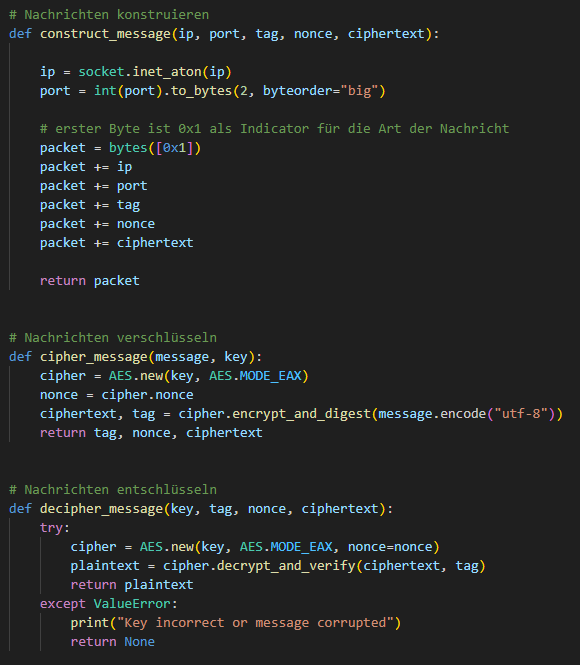
\includegraphics[width=0.5\linewidth]{picture-lib/Screenshot 2026-10-07 205225.png}
    \caption{Client.py Finale Version Abschnitt 2}
    \label{fig:A17}
\end{figure}

Auch das Empfangen von Daten musste wie auf der Serverseite stark angepasst werden. Zuerst wird geprüft, ob überhaupt Daten vorliegen, andernfalls wird der Vorgang abgebrochen. Danach wird zwischen drei Indikatoren unterschieden: Listenbefehl, Nachricht und Fehlercode.
Bei einer Nachricht mit dem Indikator 0x1 wird zuerst der Tag gelesen. Er umfasst 16 Byte ab dem achten Byte. Danach folgt der Nonce mit den nächsten 16 Byte, und alle übrigen Bytes gehören zur Nachricht. Sie wird mit \texttt{decipher\_message(\dots)} entschlüsselt und im Chatverlauf angezeigt.
Bei einer Liste mit dem Indikator 0x0 wird das erste Byte ignoriert und die Länge der übrigen Daten bestimmt. Sie werden in Blöcke von je 6 Byte aufgeteilt, wobei jeder Block die Informationen eines Benutzers enthält (IP-Adresse und Port). Diese Liste wird für die Combobox verwendet, in der der Benutzer den Empfänger auswählt. Standardmässig ist der erste Eintrag ausgewählt.
Trifft ein Fehlercode mit dem Indikator 0x2 ein, wird er im Terminal und im Chatverlauf angezeigt, damit der Benutzer weiss, dass der Empfänger nicht gefunden wurde.

\begin{figure}[H]
    \centering
    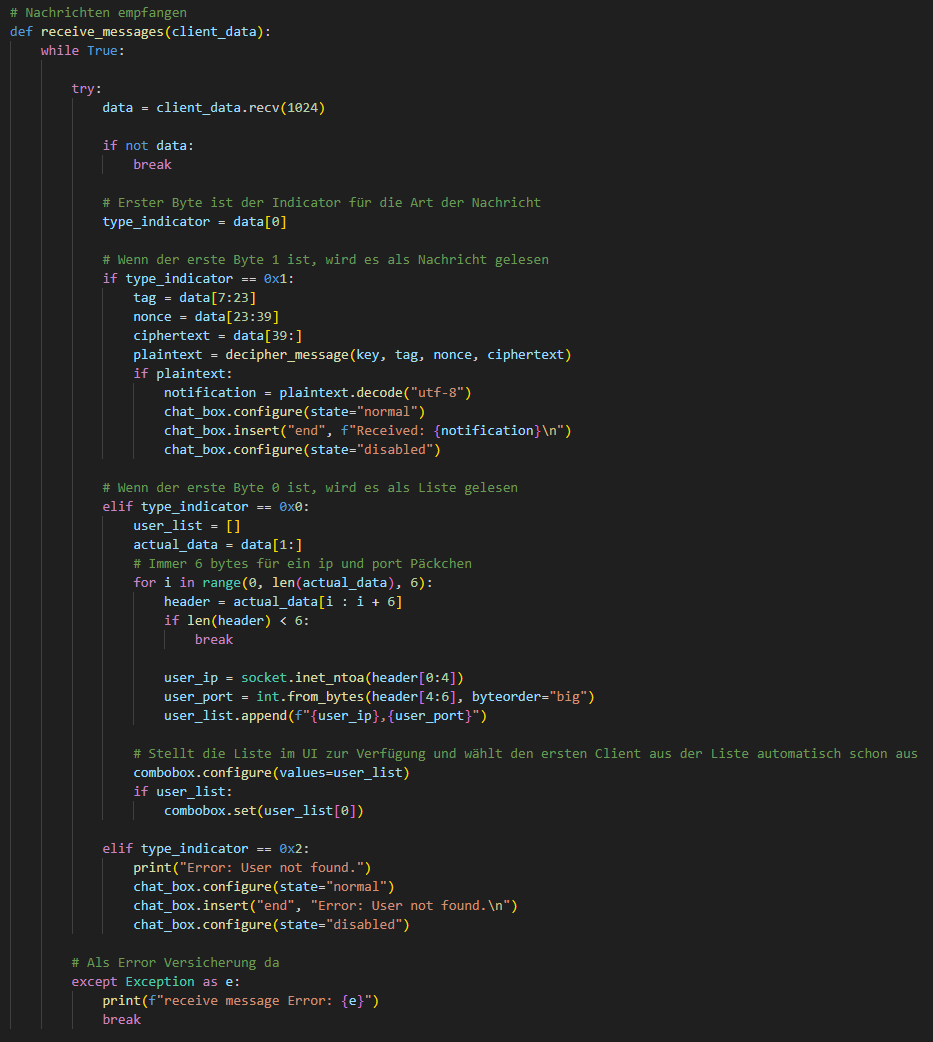
\includegraphics[width=0.75\linewidth]{picture-lib/Screenshot 2026-10-07 205237.png}
    \caption{Client.py Finale Version Abschnitt 3}
    \label{fig:A18}
\end{figure}

Die GUI wurde in einigen Punkten angepasst. Unter anderem wurde Tkinter durch die Bibliothek CustomTkinter erweitert. Sie ermöglicht ein moderneres Design mit abgerundeten Ecken und eine automatische Anpassung an das helle oder dunkle Farbschema des Computers. Weitere Einstellungen zur Anpassung sind in CustomTkinter standardmässig enthalten.

\begin{figure}[H]
    \centering
    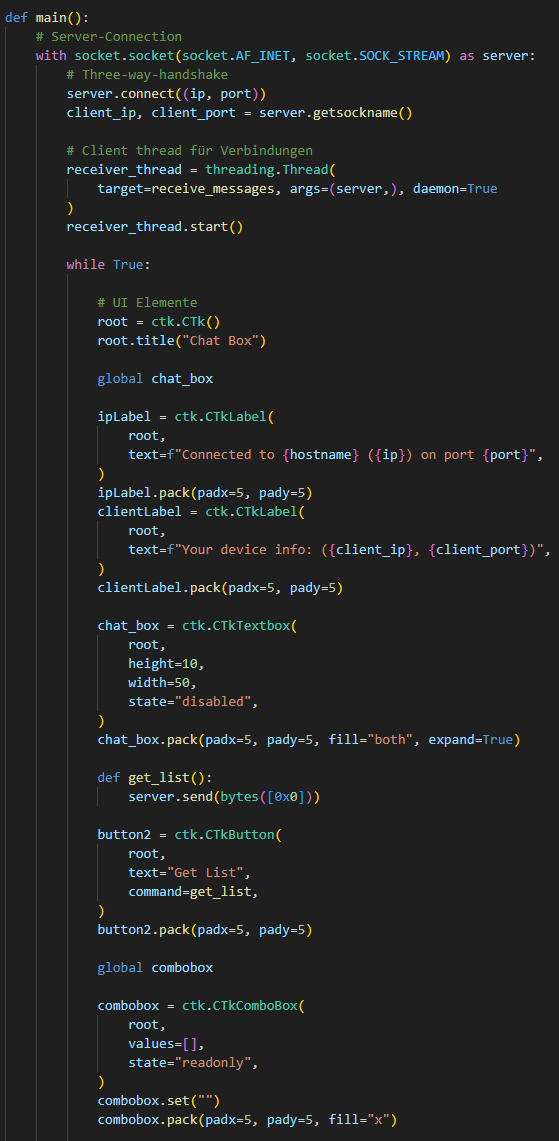
\includegraphics[width=0.5\linewidth]{picture-lib/Screenshot 2026-10-07 205316.png}
    \caption{Client.py Finale Version Abschnitt 4}
    \label{fig:A19}
\end{figure}

Die Funktion \texttt{send()} wurde ebenfalls an das Protokoll angepasst. Sie liest die benötigten Daten aus Eingabefeld und Combobox, konstruiert daraus ein Paket (\texttt{packet}) und sendet es.

\begin{figure}[H]
    \centering
    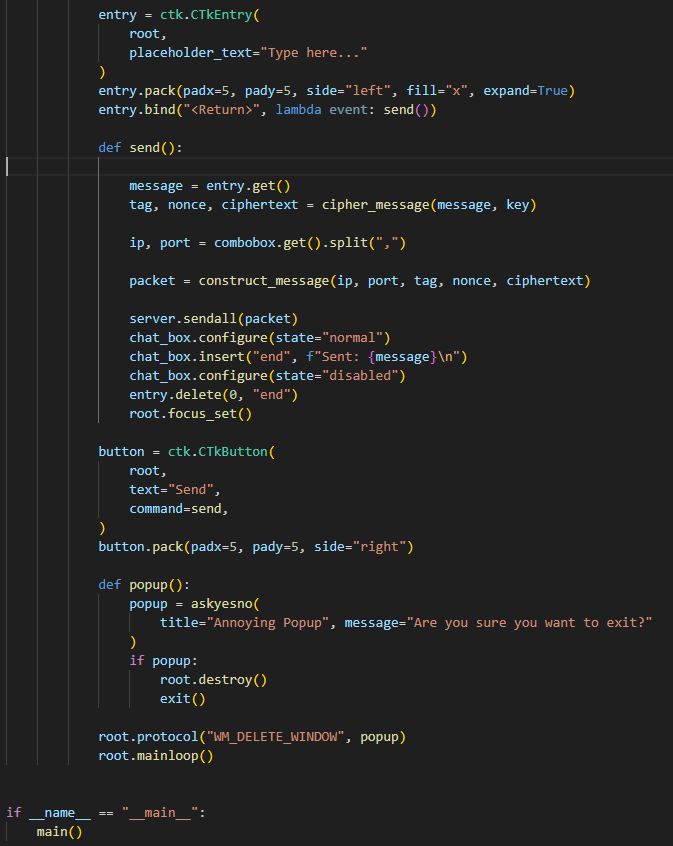
\includegraphics[width=0.5\linewidth]{picture-lib/Screenshot 2026-10-07 211314.png}
    \caption{Client.py Finale Version Abschnitt 5}
    \label{fig:A20}
\end{figure}

\subsection{Weitere Auswertungen}

Das fertige Produkt ist in Abbildung~\ref{fig:A21} zu sehen. Es zeigt den verbundenen Server sowie Informationen zur eigenen Chat Box und enthält alle Widgets, die für den Austausch einfacher Nachrichten nötig sind.

\begin{figure}[H]
    \centering
    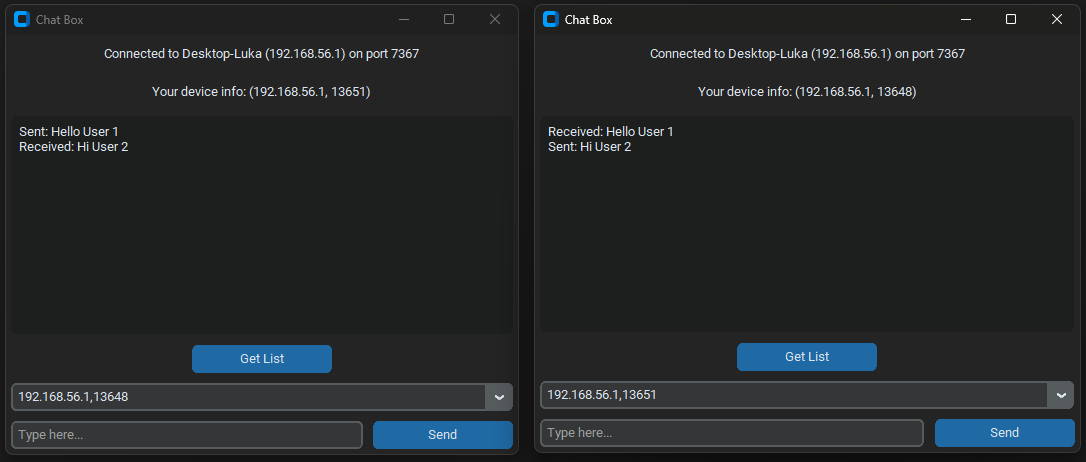
\includegraphics[width=0.75\linewidth]{picture-lib/Screenshot 2026-10-08 004928.png}
    \caption{Zwei Chat Boxen}
    \label{fig:A21}
\end{figure}

Beim Schliessen des Fensters erscheint die folgende Sicherheitsabfrage:

\begin{figure}[H]
    \centering
    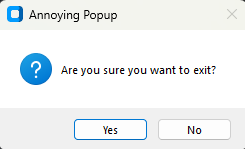
\includegraphics[width=0.5\linewidth]{picture-lib/Screenshot 2026-10-08 001339.png}
    \caption{Popup-Fenster}
    \label{fig:A22}
\end{figure}

Mit der Software Wireshark lassen sich Datenpakete in einem Netzwerk mitschneiden und auslesen.\citep{WiresharkOrg} Ich verglich eine Nachricht, die ohne Verschlüsselung gesendet wurde, mit einer verschlüsselten Nachricht. Der blau markierte Abschnitt ist in der unverschlüsselten Version (Abbildung \ref{fig:A23}) für jeden lesbar, der mit dem Netzwerk verbunden ist. In der verschlüsselten Version (Abbildung \ref{fig:A24}) besteht er nur aus Zeichen ohne erkennbaren Sinn. Erkennbar bleibt das erste Byte 01. Das ist beabsichtigt, denn es ist der Indikator [0x1], der eine Nachricht kennzeichnet. In Abbildung \ref{fig:A23} ist er nicht vorhanden.

Die Version ohne eigenes Protokoll benötigt mehr Platz für IP-Adresse und Port, da sie als umgewandelter String gesendet werden und nicht als rohe Bytes. Insgesamt benötigt die Version mit eigenem Protokoll jedoch mehr Bytes, da zusätzlich Tag und Nonce übertragen werden. Beide belegen unabhängig von der Länge der Nachricht je 16 Byte.

\begin{figure}[H]
    \centering
    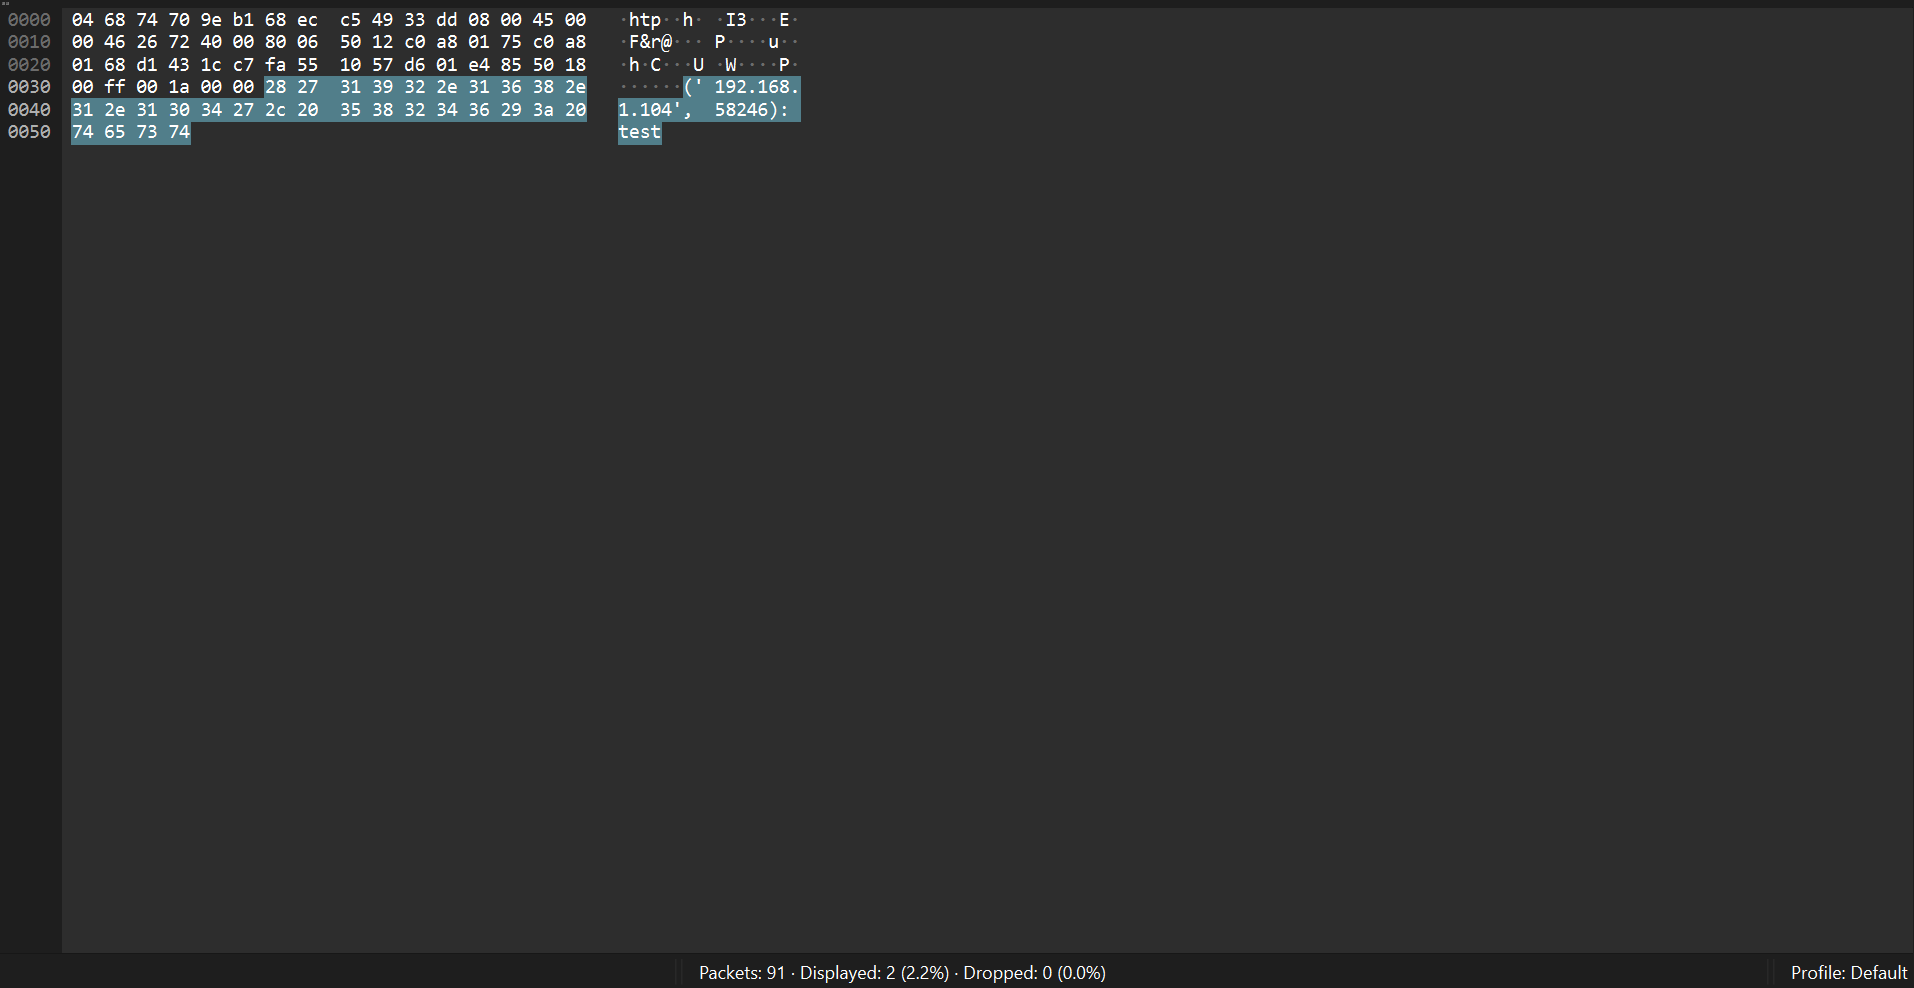
\includegraphics[width=1\linewidth]{picture-lib/Screenshot 2026-08-27 204201.png}
    \caption{Wireshark ohne Verschlüsselung und Protokoll}
    \label{fig:A23}
\end{figure}

\begin{figure}[H]
    \centering
    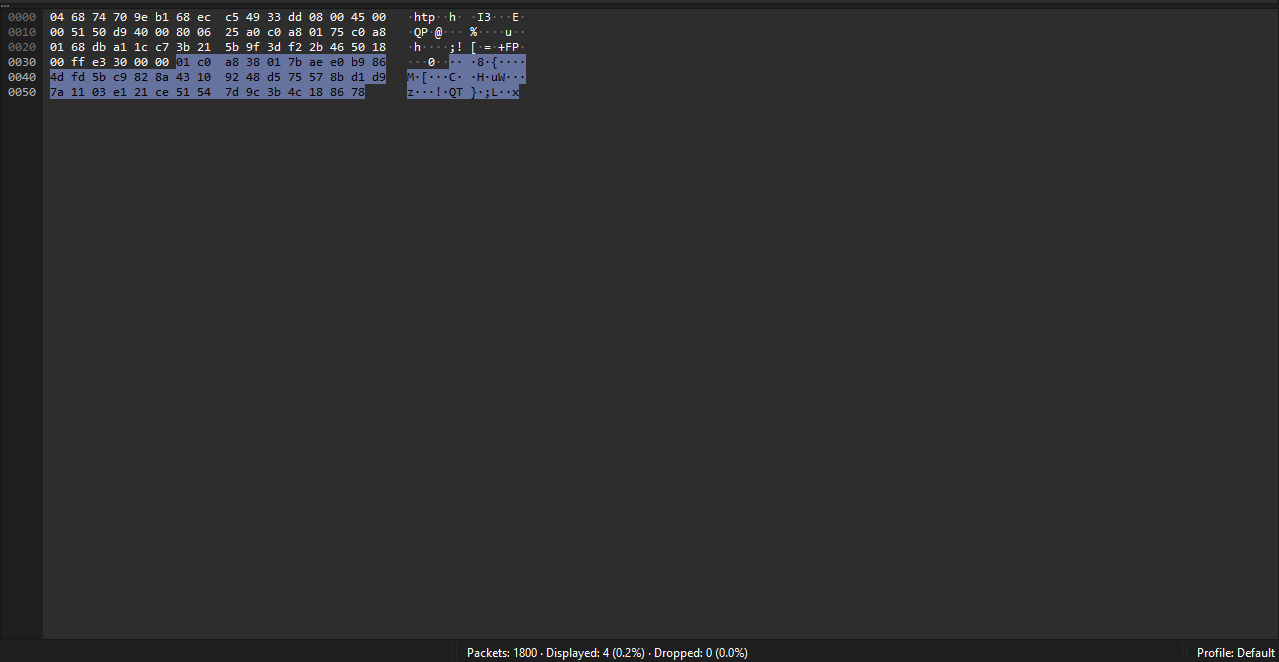
\includegraphics[width=1\linewidth]{picture-lib/Screenshot 2026-10-08 004141.png}
    \caption{Wireshark mit Verschlüsselung und Protokoll}
    \label{fig:A24}
\end{figure}

Der Inhalt der verschlüsselten Nachrichten ist mit Wireshark ohne Schlüssel nicht lesbar. Indikator, IP-Adresse und Port bleiben dagegen sichtbar, da der Server sie für die Zustellung auslesen muss. Der Verschlüsselungsvorgang beim Senden einer Nachricht ist so schnell, dass er im Betrieb nicht wahrnehmbar ist.
Die Bytes vor dem markierten Abschnitt gehören zu den Headern von TCP/IP. In beiden Abbildungen ist die erste Zeile gleich aufgebaut: \texttt{Ethernet II, Src: Intel\_XX:XX:XX (68:ec:c5:xx:xx:xx), Dst: CloudNetwork\_XX:XX:XX (04:68:74:xx:xx:xx)} beschreibt die zweite Schicht mit den MAC-Adressen von Sender und nächstem Empfänger. Sie bleiben gleich, solange dieselben Geräte miteinander kommunizieren, weil sie an die Hardware gebunden sind. Die zweite Zeile, \texttt{Internet Protocol Version 4, Src: 192.168.1.117, Dst: 192.168.1.104}, beschreibt die dritte Schicht mit den IP-Adressen. Die dritte Zeile, \texttt{Transmission Control Protocol, Src Port: 56225, Dst Port: 7367, Seq: 1, Ack: 1, Len: 41}, beschreibt TCP mit den Ports und der Länge der Nutzdaten in Bytes. Die Nutzdaten der Abbildung \ref{fig:A23} umfassen 30 Bytes, die der Abbildung \ref{fig:A24} 41 Bytes.

\chapter{Schlussfolgerung}
\label{chap:Schlussfolgerung}
Ziel meiner Arbeit war es, eine funktionsfähige Messenger-Software zu entwickeln, die verschlüsselte Nachrichten über ein selbst aufgebautes Protokoll verschickt. Bei der Umsetzung stiess ich auf mehrere Einschränkungen.
Ein vollständig eigenes Protokoll liess sich nicht realisieren. Alle Geräte kommunizieren über standardisierte Protokolle, und die Implementierung eines eigenen Protokolls hätte mehr Zeit beansprucht, als im Rahmen einer Maturaarbeit zur Verfügung steht. Zudem könnten stark veränderte Datenpakete vom Schulnetzwerk aus Sicherheitsgründen automatisch blockiert werden. Mein Protokoll betrifft deshalb nur die Nutzdaten (Payload) und wird vom TCP/IP-Protokoll gekapselt, das die Teilnehmer miteinander verbindet.
Die Implementierung entspricht ausserdem nicht dem aktuellen Stand der Technik. Sie kann Sicherheitslücken enthalten, die mir nicht bekannt sind und die sich leicht ausnutzen liessen. Damit könnten alle Benutzer gefährdet sein.
Funktional ist die Software auf Textnachrichten beschränkt, der Versand von Bildern oder Dateien wird nicht unterstützt. Um eine Verbindung aufzubauen, müssen die Verbindungsparameter in den Programmdateien manuell angepasst werden. Das Programm läuft mit Python und dem Werkzeug uv und wird über die Kommandozeile gestartet. Die grafische Benutzeroberfläche ist dagegen übersichtlich aufgebaut und einfach zu bedienen.
Ein weiterer Kritikpunkt ist, dass das Projekt keine Threading Locks verwendet, obwohl sie in der Theorie behandelt werden. Dadurch können beim Lesen und Überschreiben der Client-Liste Fehler entstehen, wenn zwei Benutzer fast gleichzeitig Änderungen vornehmen.
Ausserdem geht die Implementierung davon aus, dass ein Aufruf von \texttt{recv()} immer eine vollständige Nachricht liefert. TCP ist jedoch ein Datenstrom ohne feste Nachrichtengrenzen, deshalb könnten Nachrichten bei hoher Netzwerkauslastung unvollständig oder zusammengefasst ankommen.
Die AES-Verschlüsselung im EAX-Modus schützt zwar den Inhalt der Nachrichten vor Angreifern, gibt aber IP-Adresse und Port des Empfängers im Klartext preis. Ein Angreifer kann dadurch nachvollziehen, wer mit wem kommuniziert.

\chapter{Schlusswort}
\label{chap:Schlusswort}

\chapter{Verzeichnisse}
\label{chap:Verzeichnisse}

\nocite{*}
\printbibliography[heading=subbibnumbered]

\section{\listfigurename}
\begingroup
\makeatletter
\renewcommand{\chapter}[2]{}
\makeatother
\listoffigures
\endgroup

\section{\listtablename}
\begingroup
\makeatletter
\renewcommand{\chapter}{\@ifstar\@gobble\@gobble}
\makeatother
\listoftables
\endgroup

\section{Hilfsmittel}

Für die Arbeit habe ich folgende Hilfsmittel eingesetzt:
\begin{description}
\item[Claude Sonnet 5.5 (Antigravity)] Sprachliche Überarbeitung und Rechtschreibkorrektur der von mir selbst verfassten Texte, Hinweise auf fachliche Fehler, Formulierung der Glossareinträge sowie Hinweise zu den Quellenangaben. Die Inhalte, der Programmcode und die Argumentation habe ich selbst erarbeitet. Prompt (Auszug): "kannst du mit den Ressourcen die zur Verfügung gestellt sind bitte diesen Text so korrigieren, dass er etwas professioneller klingt und immer noch menschlich klingt."
\item[Zotero und BibTeX] Verwaltung der Quellen.
\item[Git und GitHub] Versionskontrolle und Arbeitsjournal.
\end{description}

\chapter{Anhang}
\label{chap:Anhang}

\section{Glossar}

\begin{description}
\item[AES (Advanced Encryption Standard)] Symmetrisches Verschlüsselungsverfahren, das Daten blockweise in mehreren Runden verändert.
\item[ARPANET] Vorläufer des heutigen Internets, ein Forschungsnetzwerk der USA.
\item[ASCII] Zeichenkodierung, die Zahlen Buchstaben und Zeichen zuordnet.
\item[Authentifizierung] Prüfung, ob Daten tatsächlich vom angegebenen Absender stammen und nicht verändert wurden.
\item[Backend und Frontend] Backend bezeichnet den Teil einer Software, der im Hintergrund Daten verarbeitet. Das Frontend ist die Benutzeroberfläche.
\item[Bibliothek (Library)] Sammlung von fertigem Programmcode, die in eigenen Programmen verwendet werden kann.
\item[Brute Force] Angriffsmethode, bei der alle möglichen Schlüssel systematisch durchprobiert werden.
\item[Chiffretext] Verschlüsselter, ohne Schlüssel unlesbarer Text.
\item[Client] Programm, das eine Verbindung zu einem Server aufbaut und dessen Dienste nutzt.
\item[Client-Server-Architektur] Aufbau eines Netzwerks, bei dem Clients ihre Anfragen an einen zentralen Server senden.
\item[Combobox] Auswahlfeld einer GUI, in dem man einen Eintrag aus einer Liste wählt.
\item[Daemon Thread] Thread, der im Hintergrund läuft und automatisch endet, sobald alle normalen Threads beendet sind.
\item[Datenpaket] Abgeschlossene Dateneinheit, die über ein Netzwerk verschickt wird.
\item[Diffie-Hellman-Merkle-Schlüsselaustausch] Verfahren, mit dem zwei Teilnehmer über einen offenen Kanal einen gemeinsamen geheimen Schlüssel berechnen.
\item[DNS (Domain Name System)] Dienst, der Domainnamen in IP-Adressen umwandelt.
\item[EAX-Modus] Betriebsmodus von AES, der Daten verschlüsselt und gleichzeitig authentifiziert.
\item[Endlicher Körper (Galois-Körper)] Mathematische Struktur mit endlich vielen Elementen, in der man addieren, subtrahieren, multiplizieren und dividieren kann. AES rechnet in \(\mathbb{F}_{2^8}\) mit 256 Elementen.
\item[Exploit] Programm oder Methode, die eine Sicherheitslücke ausnutzt.
\item[Flag] Statusvariable mit den Werten wahr oder falsch.
\item[Fork] Abspaltung eines bestehenden Softwareprojekts, die eigenständig weiterentwickelt oder veröffentlicht wird.
\item[Frame] Datenpaket der Sicherungsschicht mit Header und Trailer.
\item[GUI (Graphical User Interface)] Grafische Benutzeroberfläche.
\item[Header und Trailer] Zusatzinformationen vor und nach den Nutzdaten eines Datenpakets, zum Beispiel Adressen.
\item[HTTPS] Protokoll der Anwendungsschicht zur verschlüsselten Übertragung von Webseiten.
\item[Hybride Verschlüsselung] Kombination aus asymmetrischem Schlüsselaustausch und anschliessender symmetrischer Verschlüsselung.
\item[IP (Internet Protocol)] Protokoll der Vermittlungsschicht, das Datenpakete mit IP-Adressen versieht und weiterleitet.
\item[Indikator] Erstes Byte des eigenen Protokolls, das den Pakettyp angibt (0x0 Liste, 0x1 Nachricht, 0x2 Fehlercode).
\item[IP-Adresse] Eindeutige Adresse eines Geräts in einem Netzwerk.
\item[Kryptogramm] Verschlüsselter Nachrichteninhalt im eigenen Protokoll.
\item[Kryptographie] Wissenschaft der Verschlüsselung von Informationen.
\item[Lock] Sperre, die verhindert, dass mehrere Threads gleichzeitig auf dieselben Daten zugreifen.
\item[MAC-Adresse (Media Access Control)] Eindeutige Hardwareadresse einer Netzwerkkarte.
\item[Man-in-the-Middle (MitM)] Angriff, bei dem sich ein Angreifer unbemerkt in die Kommunikation zweier Teilnehmer einschaltet.
\item[Matrix] Rechteckige Anordnung von Zahlen in Zeilen und Spalten.
\item[Multithreading] Gleichzeitige Ausführung mehrerer Threads in einem Programm.
\item[Nonce (number used once)] Zufällige Zahl, die bei demselben Schlüssel nie wiederverwendet werden darf.
\item[Nutzdaten (Payload)] Eigentlicher Dateninhalt eines Pakets ohne Header und Trailer.
\item[OSI-Modell] Referenzmodell, das die Netzwerkkommunikation in sieben Schichten gliedert.
\item[Port] Nummer, die auf einem Gerät einem bestimmten Programm oder Dienst zugeordnet ist.
\item[Protokoll] Vereinbarung über Aufbau und Ablauf eines Datenaustauschs.
\item[Puffer (Buffer)] Speicherbereich, der eingehende Daten vorübergehend aufnimmt.
\item[Race Condition] Fehler, der entsteht, wenn das Ergebnis eines Programms vom zeitlichen Ablauf mehrerer Threads abhängt.
\item[Router] Gerät, das Datenpakete zwischen Netzwerken weiterleitet.
\item[Rundenschlüssel] Teilschlüssel, der aus dem AES-Schlüssel abgeleitet und in einer Runde verwendet wird.
\item[S-Box (Substitutionsbox)] Tabelle, die in AES jedes Byte durch ein anderes ersetzt.
\item[Schlüsselexpansion] Berechnung der Rundenschlüssel aus dem ursprünglichen AES-Schlüssel.
\item[Server] Programm oder Gerät, das Dienste für Clients bereitstellt.
\item[Socket] Schnittstelle des Betriebssystems für die Kommunikation über ein Netzwerk.
\item[Switch und Bridge] Geräte der Sicherungsschicht, die Netzwerkteilnehmer anhand von MAC-Adressen verbinden.
\item[Symmetrische und asymmetrische Verschlüsselung] Bei der symmetrischen Verschlüsselung verwenden beide Seiten denselben Schlüssel, bei der asymmetrischen ein Schlüsselpaar aus öffentlichem und privatem Schlüssel.
\item[Tag] Prüfwert des EAX-Modus, mit dem der Empfänger kontrolliert, ob die Nachricht unverändert ist.
\item[TCP (Transmission Control Protocol)] Zuverlässiges Protokoll der Transportschicht mit Three-Way-Handshake, Sequenzierung und Checksumme.
\item[Thread] Ausführungsstrang eines Programms.
\item[Tkinter] Python-Bibliothek für grafische Benutzeroberflächen.
\item[UDP (User Datagram Protocol)] Schnelles, aber weniger zuverlässiges Protokoll der Transportschicht.
\item[UTF-8] Zeichenkodierung, die Zeichen als Bytefolgen darstellt.
\item[uv] Werkzeug zur Verwaltung von Python-Projekten und deren Abhängigkeiten.
\item[Widget] Einzelnes Bedienelement einer GUI, zum Beispiel Schaltfläche, Eingabefeld oder Beschriftung.
\item[Wireshark] Software, die Datenpakete eines Netzwerks mitschneidet und anzeigt.
\item[XOR (exklusives Oder)] Logische Verknüpfung, die genau dann wahr ist, wenn sich die beiden Eingangswerte unterscheiden.
\item[Zotero und BibTeX] Programme zur Verwaltung von Quellen und zur Erstellung des Literaturverzeichnisses.
\end{description}

\section{Aufbau des Protokolls}
Das eigene Protokoll liegt in den Nutzdaten der TCP-Verbindung. Das erste Byte, der Indikator, bestimmt den Pakettyp.
\begin{table}[H]
    \centering
    \begin{tabular}{|l|c|c|l|}\hline
         Pakettyp & Indikator & Aufbau & Richtung\\\hline
         Liste & 0x0 & Indikator, danach je 6 Byte pro Benutzer (4 Byte IP, 2 Byte Port) & Server $\rightarrow$ Client\\\hline
         Nachricht & 0x1 & Indikator, IP, Port, Tag, Nonce, Kryptogramm & Client $\rightarrow$ Server $\rightarrow$ Client\\\hline
         Fehlercode & 0x2 & Nur Indikator, Empfänger nicht gefunden & Server $\rightarrow$ Client\\\hline
    \end{tabular}
    \caption{Pakettypen des eigenen Protokolls}
    \label{tab:A1}
\end{table}
\begin{table}[H]
    \centering
    \begin{tabular}{|l|c|c|}\hline
         Feld & Länge in Byte & Position (ab 0 gezählt)\\\hline
         Indikator & 1 & 0\\\hline
         IP-Adresse & 4 & 1 bis 4\\\hline
         Port & 2 & 5 bis 6\\\hline
         Tag & 16 & 7 bis 22\\\hline
         Nonce & 16 & 23 bis 38\\\hline
         Kryptogramm & Länge der Nachricht & ab 39\\\hline
    \end{tabular}
    \caption{Felder eines Nachrichtenpakets (0x1)}
    \label{tab:A2}
\end{table}

\section{Quellcode}
Der vollständige Quellcode aller Versionen liegt im GitHub-Repository: \url{https://github.com/Luka-Adjancic/Luka-Adjancic-Mauturaarbeit}.

\chapter{Redlichkeitserklärung}
\label{chap:Redlichkeitserklärung}

\end{document}